% Options for packages loaded elsewhere
\PassOptionsToPackage{unicode}{hyperref}
\PassOptionsToPackage{hyphens}{url}
%
\documentclass[
]{article}
\usepackage{lmodern}
\usepackage{amssymb,amsmath}
\usepackage{ifxetex,ifluatex}
\ifnum 0\ifxetex 1\fi\ifluatex 1\fi=0 % if pdftex
  \usepackage[T1]{fontenc}
  \usepackage[utf8]{inputenc}
  \usepackage{textcomp} % provide euro and other symbols
\else % if luatex or xetex
  \usepackage{unicode-math}
  \defaultfontfeatures{Scale=MatchLowercase}
  \defaultfontfeatures[\rmfamily]{Ligatures=TeX,Scale=1}
\fi
% Use upquote if available, for straight quotes in verbatim environments
\IfFileExists{upquote.sty}{\usepackage{upquote}}{}
\IfFileExists{microtype.sty}{% use microtype if available
  \usepackage[]{microtype}
  \UseMicrotypeSet[protrusion]{basicmath} % disable protrusion for tt fonts
}{}
\makeatletter
\@ifundefined{KOMAClassName}{% if non-KOMA class
  \IfFileExists{parskip.sty}{%
    \usepackage{parskip}
  }{% else
    \setlength{\parindent}{0pt}
    \setlength{\parskip}{6pt plus 2pt minus 1pt}}
}{% if KOMA class
  \KOMAoptions{parskip=half}}
\makeatother
\usepackage{xcolor}
\IfFileExists{xurl.sty}{\usepackage{xurl}}{} % add URL line breaks if available
\IfFileExists{bookmark.sty}{\usepackage{bookmark}}{\usepackage{hyperref}}
\hypersetup{
  hidelinks,
  pdfcreator={LaTeX via pandoc}}
\urlstyle{same} % disable monospaced font for URLs
\usepackage[margin=1in]{geometry}
\usepackage{graphicx,grffile}
\makeatletter
\def\maxwidth{\ifdim\Gin@nat@width>\linewidth\linewidth\else\Gin@nat@width\fi}
\def\maxheight{\ifdim\Gin@nat@height>\textheight\textheight\else\Gin@nat@height\fi}
\makeatother
% Scale images if necessary, so that they will not overflow the page
% margins by default, and it is still possible to overwrite the defaults
% using explicit options in \includegraphics[width, height, ...]{}
\setkeys{Gin}{width=\maxwidth,height=\maxheight,keepaspectratio}
% Set default figure placement to htbp
\makeatletter
\def\fps@figure{htbp}
\makeatother
\setlength{\emergencystretch}{3em} % prevent overfull lines
\providecommand{\tightlist}{%
  \setlength{\itemsep}{0pt}\setlength{\parskip}{0pt}}
\setcounter{secnumdepth}{-\maxdimen} % remove section numbering
%latex header to wrap code lines in .pdf

\usepackage{fvextra}
\DefineVerbatimEnvironment{Highlighting}{Verbatim}{breaklines,commandchars=\\\{\}}

% To keep the figure from floating around
% All figures should be forced in-place via the [H]ERE float specification.
\usepackage{float}
\floatplacement{figure}{H}
%\floatplacement{figure}{!htbp}

\date{}

\begin{document}

\hypertarget{report-of-the-fit}{%
\section{Report of the fit}\label{report-of-the-fit}}

\hypertarget{fit-summary}{%
\subsection{Fit summary}\label{fit-summary}}

Description: PV19 version x, parameters for NNLL. Initial parameters
from a previous fit with ceres on replica zero. T0 parameters from the
previous to previous fit. Steps from minuit minimisation.\\
Minimiser: minuit\\
Random seed: 1234\\
Maximum values allowed for \(q_T / Q\): 0.2\\
Cut on the error function: 4\\
Parameterisation: PV19x\\
Explicit formula:

\[f_{\rm NP}(x,\zeta, b_T)= \Biggl(
\frac{1-\lambda}{1 + g_1(x) b_T^2/4} + \lambda \exp \left(-g_{1B}(x) b_T^2 / 4 \right)\Biggr) \exp\left[- g_2 \log\left(\frac{\zeta}{Q_0^2}\right) b_T^2/4 - g_{2B} \log\left(\frac{\zeta}{Q_0^2}\right) b_T^4/4 \right]\]\[g_1(x) = \frac{N_1}{x\sigma} \exp\left[ - \frac{\ln^2\left(\frac{x}{\alpha}\right)}{2 \sigma^2} \right]\]\[g_{1B}(x) = \frac{N_{1B}}{x\sigma_B} \exp\left[ - \frac{\ln^2\left(\frac{x}{\alpha_B}\right)}{2 \sigma_B^2} \right]\]\[Q_0^2 = 1\;{\rm GeV}^2\]
\(t_0\) prescription: True

\begin{table}[h]

\centering

\begin{tabular}{|c|c|c|c|c|c|c|c|c|} \hline

\textbf{\(g_2\)} & \textbf{\(N_1\)} & \textbf{\(\alpha\)} & \textbf{\(\sigma\)} & \textbf{\(\lambda\)} & \textbf{\(N_{1B}\)} & \textbf{\(\alpha_B\)} & \textbf{\(\sigma_B\)} & \textbf{\(g_{2B}\)} \\ \hline

0.005144 & 0.68535248 & 0.21943481 & 0.3329461 & 0.66627605 & 0.0387879 & 0.075758463 & 0.34845635 & 0.019224141 \\ \hline

\end{tabular}

\caption{}

\end{table}

\hypertarget{theory-summary}{%
\subsection{Theory summary}\label{theory-summary}}

Collinear PDF set: MMHT2014nlo68cl member 0\\
Collinear FF set: DSS14\_NLO\_PiSum member 0\\
\(b^*\) prescription: bstarmin\\
Perturbative order: NNLL\\
Initial parameters fluctuations: True\\
Reference value of the fine-structure constant:
\(\alpha(Q = 91.1876\;{\rm GeV}) = 0.00776578395589\) (running True)

\hypertarget{global-statistical-estimators}{%
\subsection{Global statistical
estimators}\label{global-statistical-estimators}}

\(N_{rep}\) = 173\\
\(\chi_{0}^2\) = 1.6571\\
\(\chi_{mean}^2\) = 1.6341\\
\(\langle\chi^2\rangle \pm \sigma_{\chi^2}\) = 1.6823 \(\pm\) 0.0163\\
\(\langle E \rangle \pm \sigma_{E}\) = 2.6372 \(\pm\) 0.1915

\hypertarget{parameters}{%
\subsection{Parameters}\label{parameters}}

\begin{table}[h]

\centering

\begin{tabular}{|c|c|c|c|} \hline

\textbf{Parameter} & \textbf{Central replica} & \textbf{Average over
replicas} & \textbf{Fixed} \\ \hline

\(g_2\) & -0.091343204 & -0.09242544 \(\pm\)
0.01642545 & False \\ \hline
\(N_1\) & 5.3553982 & 5.3553982 \(\pm\) 0.0 & True \\ \hline
\(\alpha\) & 1.0805391 & 1.09779861 \(\pm\) 0.38066408 & False \\ \hline
\(\sigma\) & 0.9431266 & 0.91765216 \(\pm\) 0.12484923 & False \\ \hline
\(\lambda\) & 0.49120348 & 0.48996388 \(\pm\)
0.07100341 & False \\ \hline
\(N_{1B}\) & 0.040471695 & 0.04404218 \(\pm\)
0.01034721 & False \\ \hline
\(\alpha_B\) & 0.052405509 & 0.05811231 \(\pm\)
0.02975318 & False \\ \hline
\(\sigma_B\) & 0.56591202 & 0.53112528 \(\pm\)
0.11609349 & False \\ \hline
\(g_{2B}\) & 0.034188315 & 0.03495914 \(\pm\)
0.00804642 & False \\ \hline

\end{tabular}

\caption{}

\end{table}

\begin{figure}
\centering
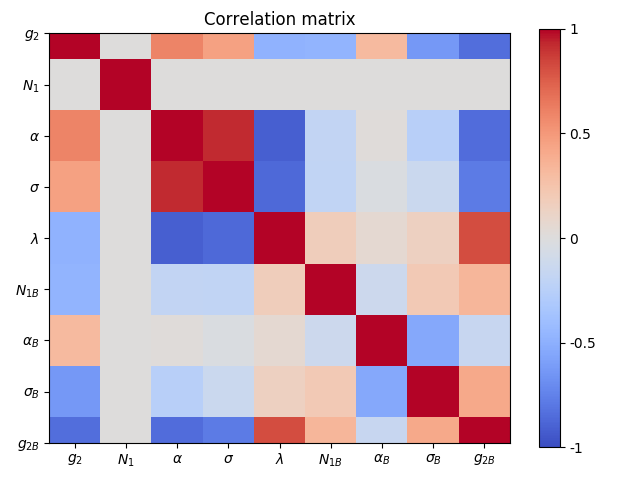
\includegraphics{pngplots/CorrelationMatrix.png}
\caption{Fitted parameter correlation matrix}
\end{figure}

\hypertarget{fit-properties}{%
\subsection{Fit properties}\label{fit-properties}}

\begin{figure}
\centering
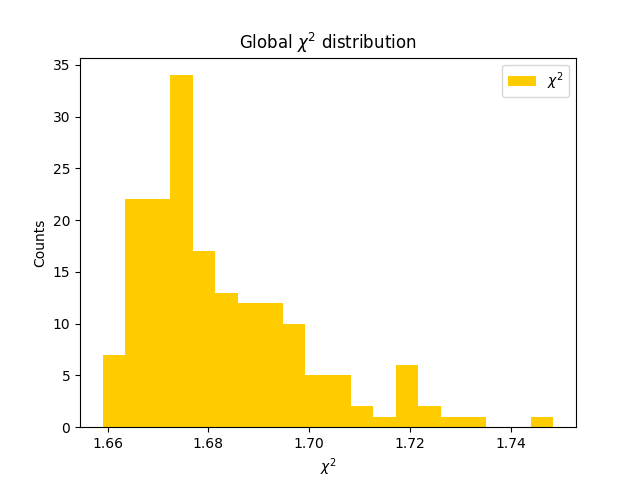
\includegraphics{pngplots/Globalchi2.png}
\caption{Global \(\chi^2\) distribution}
\end{figure}

\begin{figure}
\centering
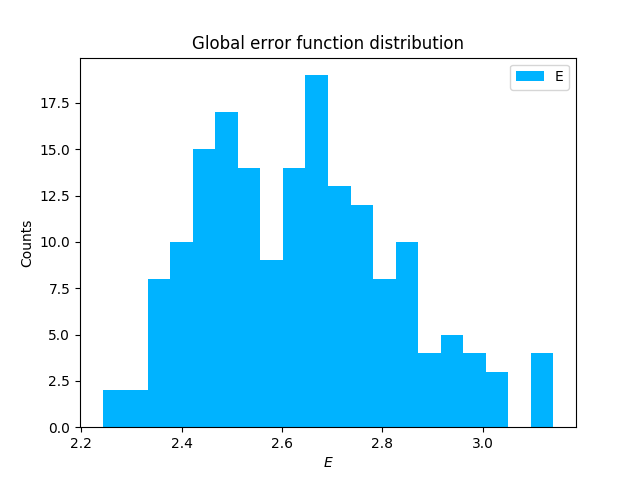
\includegraphics{pngplots/GlobalErrorFunction.png}
\caption{Global error function distribution}
\end{figure}

\begin{figure}
\centering
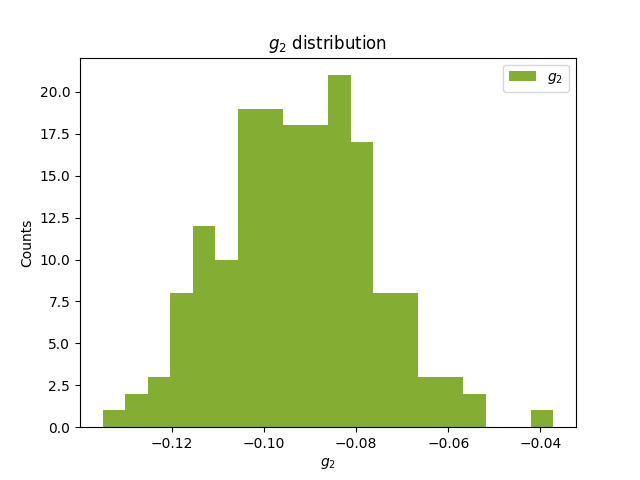
\includegraphics{pngplots/param0.png}
\caption{\(g_2\) distribution}
\end{figure}

\begin{figure}
\centering
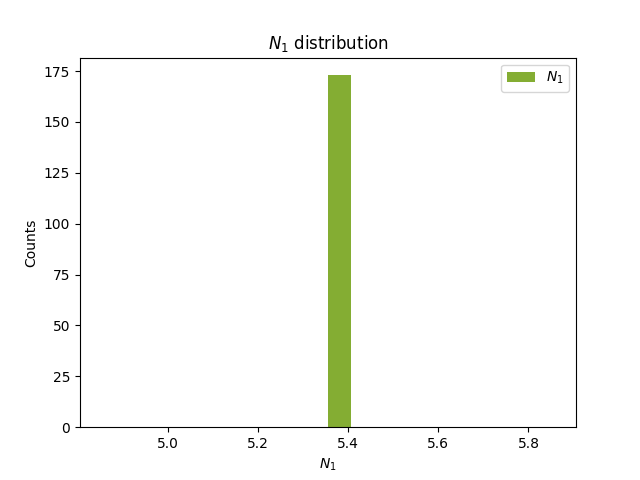
\includegraphics{pngplots/param1.png}
\caption{\(N_1\) distribution}
\end{figure}

\begin{figure}
\centering
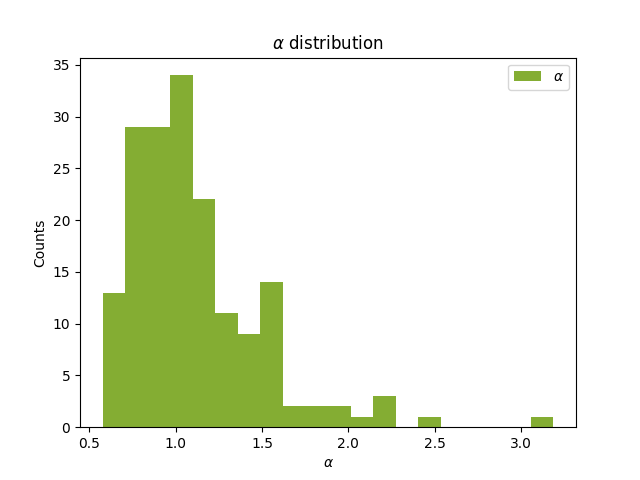
\includegraphics{pngplots/param2.png}
\caption{\(\alpha\) distribution}
\end{figure}

\begin{figure}
\centering
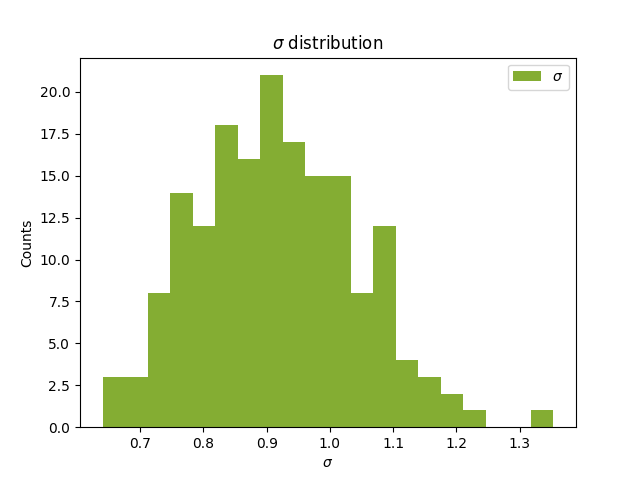
\includegraphics{pngplots/param3.png}
\caption{\(\sigma\) distribution}
\end{figure}

\begin{figure}
\centering
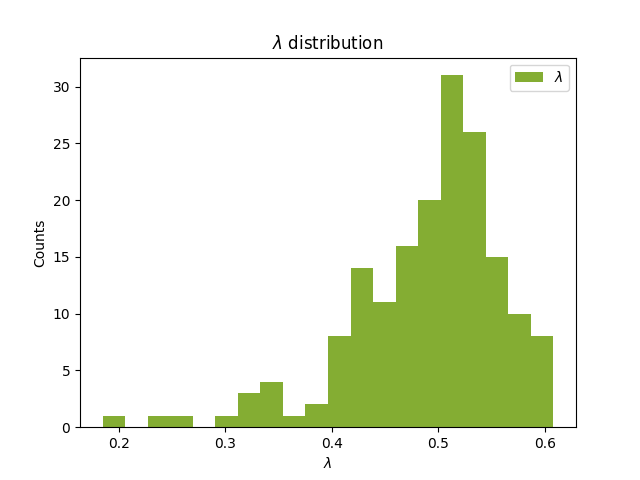
\includegraphics{pngplots/param4.png}
\caption{\(\lambda\) distribution}
\end{figure}

\begin{figure}
\centering
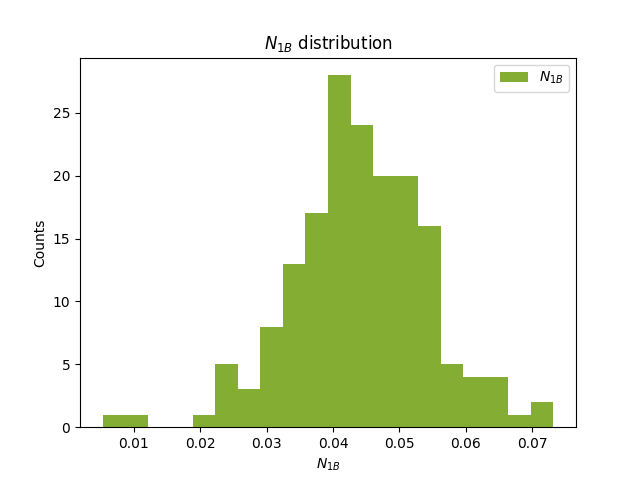
\includegraphics{pngplots/param5.png}
\caption{\(N_{1B}\) distribution}
\end{figure}

\begin{figure}
\centering
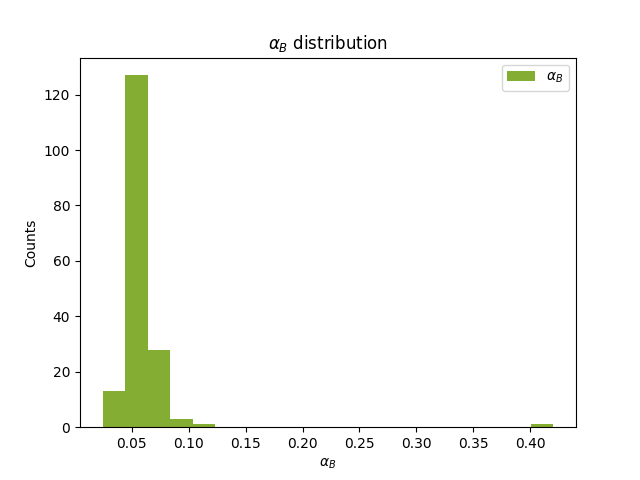
\includegraphics{pngplots/param6.png}
\caption{\(\alpha_B\) distribution}
\end{figure}

\begin{figure}
\centering
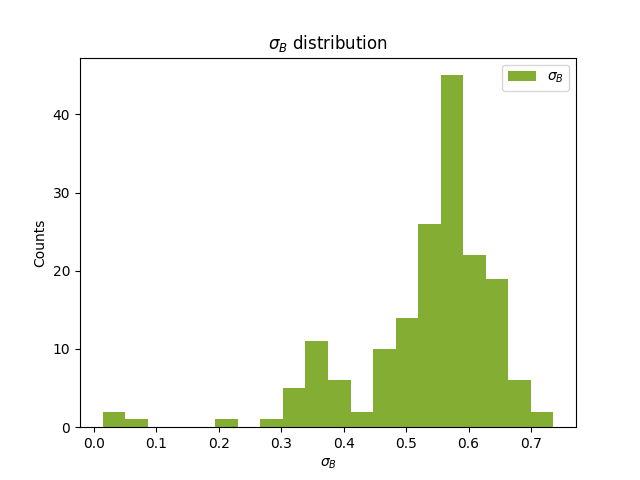
\includegraphics{pngplots/param7.png}
\caption{\(\sigma_B\) distribution}
\end{figure}

\begin{figure}
\centering
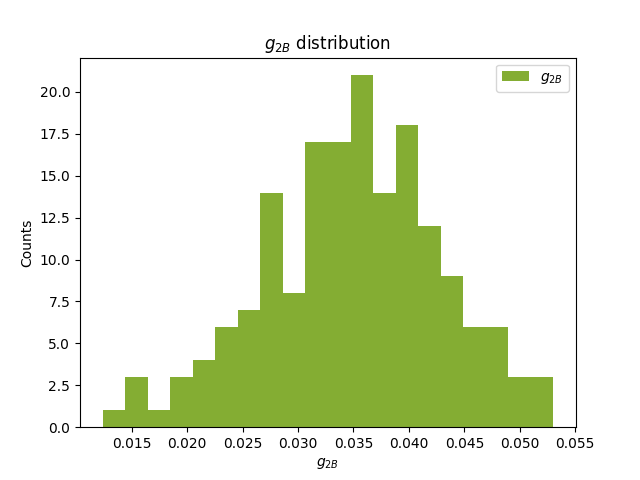
\includegraphics{pngplots/param8.png}
\caption{\(g_{2B}\) distribution}
\end{figure}

\hypertarget{table-of-chi2s}{%
\subsection{\texorpdfstring{Table of
\(\chi^2\)'s}{Table of \textbackslash chi\^{}2's}}\label{table-of-chi2s}}

\begin{table}[h]

\centering

\begin{tabular}{|c|c|c|c|c|} \hline

\textbf{Experiment} & \textbf{Number of
points} & \textbf{\(\chi_{D}^2\)} & \textbf{\(\chi_{\lambda}^2\)} & \textbf{\(\chi^2\)} \\ \hline

E605\_Q\_7\_8 & 7 & 0.4826 & 0.0313 & 0.514 \\ \hline
E605\_Q\_8\_9 & 8 & 0.9991 & 0.0179 & 1.017 \\ \hline
E605\_Q\_10.5\_11.5 & 10 & 0.4928 & 0.1393 & 0.6322 \\ \hline
E288\_200\_Q\_4\_5 & 4 & 0.9256 & 0.8564 & 1.782 \\ \hline
E288\_200\_Q\_5\_6 & 5 & 2.3052 & 0.3541 & 2.6593 \\ \hline
E288\_200\_Q\_6\_7 & 6 & 0.7917 & 0.2111 & 1.0028 \\ \hline
E288\_200\_Q\_7\_8 & 7 & 0.9857 & 0.032 & 1.0177 \\ \hline
E288\_200\_Q\_8\_9 & 8 & 0.7347 & 0.0059 & 0.7406 \\ \hline
E288\_300\_Q\_4\_5 & 4 & 0.7749 & 0.3398 & 1.1147 \\ \hline
E288\_300\_Q\_5\_6 & 5 & 1.394 & 0.0995 & 1.4935 \\ \hline
E288\_300\_Q\_6\_7 & 6 & 1.0371 & 0.0397 & 1.0768 \\ \hline
E288\_300\_Q\_7\_8 & 7 & 0.3419 & 0.0425 & 0.3844 \\ \hline
E288\_300\_Q\_8\_9 & 8 & 0.3924 & 0.0384 & 0.4308 \\ \hline
E288\_400\_Q\_5\_6 & 5 & 0.9363 & 0.0011 & 0.9374 \\ \hline
E288\_400\_Q\_6\_7 & 6 & 0.5219 & 0.0069 & 0.5287 \\ \hline
E288\_400\_Q\_7\_8 & 7 & 0.2461 & 0.0139 & 0.26 \\ \hline
E288\_400\_Q\_8\_9 & 8 & 0.5589 & 0.0127 & 0.5716 \\ \hline
E288\_400\_Q\_11\_12 & 11 & 0.5713 & 0.0068 & 0.5781 \\ \hline
E288\_400\_Q\_12\_13 & 12 & 0.5368 & 0.0113 & 0.5481 \\ \hline
E288\_400\_Q\_13\_14 & 12 & 0.3425 & 0.0362 & 0.3787 \\ \hline
STAR\_510 & 7 & 1.193 & 0.0135 & 1.2066 \\ \hline
CDF\_RunI & 25 & 0.6526 & 0.1483 & 0.8009 \\ \hline
CDF\_RunII & 26 & 1.2796 & 0.0074 & 1.287 \\ \hline
D0\_RunI & 12 & 0.6669 & 0.0018 & 0.6687 \\ \hline
D0\_RunII & 5 & 0.914 & 0.2909 & 1.2049 \\ \hline
D0\_RunIImu & 3 & 0.1228 & 0.0862 & 0.2089 \\ \hline
LHCb\_7TeV & 7 & 1.9434 & 0.8425 & 2.7859 \\ \hline
LHCb\_8TeV & 7 & 1.9152 & 1.452 & 3.3672 \\ \hline
LHCb\_13TeV & 7 & 1.4916 & 0.2891 & 1.7807 \\ \hline
CMS\_7TeV & 4 & 2.8935 & 0 & 2.8935 \\ \hline
CMS\_8TeV & 4 & 1.4855 & 0.1783 & 1.6639 \\ \hline
ATLAS\_7TeV\_y\_0\_1 & 6 & 6.9605 & 1.0906 & 8.0511 \\ \hline
ATLAS\_7TeV\_y\_1\_2 & 6 & 4.9357 & 0.4829 & 5.4186 \\ \hline
ATLAS\_7TeV\_y\_2\_2.4 & 6 & 1.8106 & 0.0099 & 1.8206 \\ \hline
ATLAS\_8TeV\_y\_0\_0.4 & 6 & 4.7809 & 0.9768 & 5.7576 \\ \hline
ATLAS\_8TeV\_y\_0.4\_0.8 & 6 & 6.7037 & 1.5463 & 8.2501 \\ \hline
ATLAS\_8TeV\_y\_0.8\_1.2 & 6 & 4.364 & 0.6694 & 5.0335 \\ \hline
ATLAS\_8TeV\_y\_1.2\_1.6 & 6 & 2.9492 & 0.4253 & 3.3745 \\ \hline
ATLAS\_8TeV\_y\_1.6\_2 & 6 & 2.5631 & 0.2704 & 2.8336 \\ \hline
ATLAS\_8TeV\_y\_2\_2.4 & 6 & 1.2871 & 0.162 & 1.449 \\ \hline
ATLAS\_8TeV\_Q\_46\_66 & 4 & 0.7702 & 0.0369 & 0.8071 \\ \hline
ATLAS\_8TeV\_Q\_116\_150 & 8 & 1.1515 & 0.0073 & 1.1587 \\ \hline
Total & 319 & - & - & 1.6571 \\ \hline

\end{tabular}

\caption{Central-replica \(\chi^2\)'s:}

\end{table}

\begin{table}[h]

\centering

\begin{tabular}{|c|c|c|c|c|} \hline

\textbf{Experiment} & \textbf{Number of
points} & \textbf{\(\chi_{D}^2\)} & \textbf{\(\chi_{\lambda}^2\)} & \textbf{\(\chi^2\)} \\ \hline

E605\_Q\_7\_8 & 7 & 0.6195 & 0.0842 & 0.7037 \\ \hline
E605\_Q\_8\_9 & 8 & 1.2033 & 0.0491 & 1.2524 \\ \hline
E605\_Q\_10.5\_11.5 & 10 & 0.3704 & 0.0966 & 0.467 \\ \hline
E288\_200\_Q\_4\_5 & 4 & 0.4592 & 0.4626 & 0.9218 \\ \hline
E288\_200\_Q\_5\_6 & 5 & 1.3421 & 0.2805 & 1.6226 \\ \hline
E288\_200\_Q\_6\_7 & 6 & 0.5894 & 0.1838 & 0.7731 \\ \hline
E288\_200\_Q\_7\_8 & 7 & 0.9044 & 0.0379 & 0.9423 \\ \hline
E288\_200\_Q\_8\_9 & 8 & 0.9133 & 0.009 & 0.9223 \\ \hline
E288\_300\_Q\_4\_5 & 4 & 0.5417 & 0.1742 & 0.7159 \\ \hline
E288\_300\_Q\_5\_6 & 5 & 1.1792 & 0.0622 & 1.2414 \\ \hline
E288\_300\_Q\_6\_7 & 6 & 0.9837 & 0.0266 & 1.0104 \\ \hline
E288\_300\_Q\_7\_8 & 7 & 0.3435 & 0.0331 & 0.3766 \\ \hline
E288\_300\_Q\_8\_9 & 8 & 0.2798 & 0.0403 & 0.3201 \\ \hline
E288\_400\_Q\_5\_6 & 5 & 1.1387 & 0.0151 & 1.1538 \\ \hline
E288\_400\_Q\_6\_7 & 6 & 0.6721 & 0.0307 & 0.7028 \\ \hline
E288\_400\_Q\_7\_8 & 7 & 0.3372 & 0.0486 & 0.3857 \\ \hline
E288\_400\_Q\_8\_9 & 8 & 0.7678 & 0.0428 & 0.8106 \\ \hline
E288\_400\_Q\_11\_12 & 11 & 0.843 & 0.0125 & 0.8555 \\ \hline
E288\_400\_Q\_12\_13 & 12 & 0.8667 & 0.0144 & 0.8812 \\ \hline
E288\_400\_Q\_13\_14 & 12 & 0.8896 & 0.0579 & 0.9475 \\ \hline
STAR\_510 & 7 & 1.1585 & 0.0374 & 1.1959 \\ \hline
CDF\_RunI & 25 & 0.5704 & 0.1422 & 0.7126 \\ \hline
CDF\_RunII & 26 & 1.2159 & 0.006 & 1.2219 \\ \hline
D0\_RunI & 12 & 0.6306 & 0.0007 & 0.6313 \\ \hline
D0\_RunII & 5 & 1.0627 & 0.2934 & 1.3561 \\ \hline
D0\_RunIImu & 3 & 0.0272 & 0.0358 & 0.063 \\ \hline
LHCb\_7TeV & 7 & 1.661 & 0.8488 & 2.5097 \\ \hline
LHCb\_8TeV & 7 & 1.7915 & 1.3835 & 3.175 \\ \hline
LHCb\_13TeV & 7 & 1.344 & 0.2686 & 1.6126 \\ \hline
CMS\_7TeV & 4 & 2.8712 & 0 & 2.8712 \\ \hline
CMS\_8TeV & 4 & 1.4974 & 0.1813 & 1.6787 \\ \hline
ATLAS\_7TeV\_y\_0\_1 & 6 & 6.8994 & 1.096 & 7.9954 \\ \hline
ATLAS\_7TeV\_y\_1\_2 & 6 & 4.7533 & 0.4859 & 5.2392 \\ \hline
ATLAS\_7TeV\_y\_2\_2.4 & 6 & 1.6877 & 0.0099 & 1.6977 \\ \hline
ATLAS\_8TeV\_y\_0\_0.4 & 6 & 4.738 & 1.0098 & 5.7477 \\ \hline
ATLAS\_8TeV\_y\_0.4\_0.8 & 6 & 6.4935 & 1.5968 & 8.0902 \\ \hline
ATLAS\_8TeV\_y\_0.8\_1.2 & 6 & 4.3266 & 0.6857 & 5.0122 \\ \hline
ATLAS\_8TeV\_y\_1.2\_1.6 & 6 & 2.9076 & 0.4354 & 3.3429 \\ \hline
ATLAS\_8TeV\_y\_1.6\_2 & 6 & 2.4013 & 0.2642 & 2.6655 \\ \hline
ATLAS\_8TeV\_y\_2\_2.4 & 6 & 1.1461 & 0.1525 & 1.2986 \\ \hline
ATLAS\_8TeV\_Q\_46\_66 & 4 & 0.7042 & 0.0484 & 0.7526 \\ \hline
ATLAS\_8TeV\_Q\_116\_150 & 8 & 1.1248 & 0.0066 & 1.1314 \\ \hline
Total & 319 & - & - & 1.6341 \\ \hline

\end{tabular}

\caption{Mean-replica \(\chi^2\)'s:}

\end{table}

\begin{table}[h]

\centering

\begin{tabular}{|c|c|c|c|c|} \hline

\textbf{Experiment} & \textbf{Number of
points} & \textbf{\(\chi_{D}^2\)} & \textbf{\(\chi_{\lambda}^2\)} & \textbf{\(\chi^2\)} \\ \hline

E605\_Q\_7\_8 & 7 & 0.4012 \(\pm\) 0.196 & 0.1483 \(\pm\)
0.1924 & 0.5495 \(\pm\) 0.0847 \\ \hline
E605\_Q\_8\_9 & 8 & 1.0003 \(\pm\) 0.2367 & 0.0859 \(\pm\)
0.1279 & 1.0862 \(\pm\) 0.2086 \\ \hline
E605\_Q\_10.5\_11.5 & 10 & 0.4673 \(\pm\) 0.2605 & 0.2056 \(\pm\)
0.2478 & 0.6728 \(\pm\) 0.0761 \\ \hline
E288\_200\_Q\_4\_5 & 4 & 0.5306 \(\pm\) 1.2697 & 1.2825 \(\pm\)
1.266 & 1.8131 \(\pm\) 0.2217 \\ \hline
E288\_200\_Q\_5\_6 & 5 & 2.1727 \(\pm\) 0.6684 & 0.4979 \(\pm\)
0.6223 & 2.6706 \(\pm\) 0.2632 \\ \hline
E288\_200\_Q\_6\_7 & 6 & 0.6727 \(\pm\) 0.4411 & 0.3413 \(\pm\)
0.3939 & 1.014 \(\pm\) 0.1729 \\ \hline
E288\_200\_Q\_7\_8 & 7 & 0.9237 \(\pm\) 0.2413 & 0.1062 \(\pm\)
0.1425 & 1.0299 \(\pm\) 0.1998 \\ \hline
E288\_200\_Q\_8\_9 & 8 & 0.688 \(\pm\) 0.1183 & 0.064 \(\pm\)
0.0755 & 0.752 \(\pm\) 0.0997 \\ \hline
E288\_300\_Q\_4\_5 & 4 & 0.5549 \(\pm\) 0.7565 & 0.5879 \(\pm\)
0.7068 & 1.1428 \(\pm\) 0.185 \\ \hline
E288\_300\_Q\_5\_6 & 5 & 1.2346 \(\pm\) 0.4592 & 0.2725 \(\pm\)
0.3725 & 1.5071 \(\pm\) 0.2395 \\ \hline
E288\_300\_Q\_6\_7 & 6 & 0.9221 \(\pm\) 0.3494 & 0.1676 \(\pm\)
0.2324 & 1.0896 \(\pm\) 0.2635 \\ \hline
E288\_300\_Q\_7\_8 & 7 & 0.2477 \(\pm\) 0.2349 & 0.1536 \(\pm\)
0.1913 & 0.4012 \(\pm\) 0.137 \\ \hline
E288\_300\_Q\_8\_9 & 8 & 0.3315 \(\pm\) 0.1806 & 0.1181 \(\pm\)
0.179 & 0.4496 \(\pm\) 0.0463 \\ \hline
E288\_400\_Q\_5\_6 & 5 & 0.8122 \(\pm\) 0.3319 & 0.1509 \(\pm\)
0.205 & 0.963 \(\pm\) 0.264 \\ \hline
E288\_400\_Q\_6\_7 & 6 & 0.4678 \(\pm\) 0.2964 & 0.1032 \(\pm\)
0.1282 & 0.571 \(\pm\) 0.2674 \\ \hline
E288\_400\_Q\_7\_8 & 7 & 0.2127 \(\pm\) 0.269 & 0.1056 \(\pm\)
0.1538 & 0.3184 \(\pm\) 0.2222 \\ \hline
E288\_400\_Q\_8\_9 & 8 & 0.5501 \(\pm\) 0.1788 & 0.0772 \(\pm\)
0.1165 & 0.6274 \(\pm\) 0.1502 \\ \hline
E288\_400\_Q\_11\_12 & 11 & 0.5719 \(\pm\) 0.131 & 0.0414 \(\pm\)
0.055 & 0.6132 \(\pm\) 0.1358 \\ \hline
E288\_400\_Q\_12\_13 & 12 & 0.5431 \(\pm\) 0.0747 & 0.0394 \(\pm\)
0.0527 & 0.5825 \(\pm\) 0.0703 \\ \hline
E288\_400\_Q\_13\_14 & 12 & 0.3493 \(\pm\) 0.1013 & 0.0564 \(\pm\)
0.0544 & 0.4057 \(\pm\) 0.0953 \\ \hline
STAR\_510 & 7 & 1.0834 \(\pm\) 0.2123 & 0.1266 \(\pm\) 0.1987 & 1.2099
\(\pm\) 0.0741 \\ \hline
CDF\_RunI & 25 & 0.6151 \(\pm\) 0.1782 & 0.1935 \(\pm\) 0.176 & 0.8086
\(\pm\) 0.0292 \\ \hline
CDF\_RunII & 26 & 1.2818 \(\pm\) 0.2061 & 0.0594 \(\pm\) 0.0782 & 1.3412
\(\pm\) 0.1926 \\ \hline
D0\_RunI & 12 & 0.606 \(\pm\) 0.118 & 0.0671 \(\pm\) 0.0903 & 0.6731
\(\pm\) 0.0658 \\ \hline
D0\_RunII & 5 & 0.7417 \(\pm\) 0.6179 & 0.4881 \(\pm\) 0.5955 & 1.2298
\(\pm\) 0.2071 \\ \hline
D0\_RunIImu & 3 & -0.4071 \(\pm\) 0.6127 & 0.6123 \(\pm\)
0.5833 & 0.2052 \(\pm\) 0.148 \\ \hline
LHCb\_7TeV & 7 & 1.7025 \(\pm\) 0.7706 & 1.1015 \(\pm\) 0.7533 & 2.8039
\(\pm\) 0.1105 \\ \hline
LHCb\_8TeV & 7 & 1.9122 \(\pm\) 1.0007 & 1.5449 \(\pm\) 0.9398 & 3.4572
\(\pm\) 0.3265 \\ \hline
LHCb\_13TeV & 7 & 1.4642 \(\pm\) 0.3904 & 0.3374 \(\pm\) 0.3847 & 1.8016
\(\pm\) 0.0951 \\ \hline
CMS\_7TeV & 4 & 2.8904 \(\pm\) 0.0257 & 0.0 \(\pm\) 0.0 & 2.8904 \(\pm\)
0.0257 \\ \hline
CMS\_8TeV & 4 & 1.3955 \(\pm\) 0.2499 & 0.2567 \(\pm\) 0.2426 & 1.6522
\(\pm\) 0.0817 \\ \hline
ATLAS\_7TeV\_y\_0\_1 & 6 & 6.8515 \(\pm\) 0.6888 & 1.1929 \(\pm\)
0.5544 & 8.0444 \(\pm\) 0.3425 \\ \hline
ATLAS\_7TeV\_y\_1\_2 & 6 & 4.8939 \(\pm\) 0.4218 & 0.5516 \(\pm\)
0.3337 & 5.4455 \(\pm\) 0.3158 \\ \hline
ATLAS\_7TeV\_y\_2\_2.4 & 6 & 1.795 \(\pm\) 0.1024 & 0.0259 \(\pm\)
0.0376 & 1.8208 \(\pm\) 0.0947 \\ \hline
ATLAS\_8TeV\_y\_0\_0.4 & 6 & 4.7816 \(\pm\) 0.5525 & 1.0105 \(\pm\)
0.4893 & 5.792 \(\pm\) 0.2334 \\ \hline
ATLAS\_8TeV\_y\_0.4\_0.8 & 6 & 6.6527 \(\pm\) 0.7791 & 1.6466 \(\pm\)
0.7575 & 8.2993 \(\pm\) 0.2469 \\ \hline
ATLAS\_8TeV\_y\_0.8\_1.2 & 6 & 4.2661 \(\pm\) 0.4391 & 0.7099 \(\pm\)
0.3556 & 4.976 \(\pm\) 0.1986 \\ \hline
ATLAS\_8TeV\_y\_1.2\_1.6 & 6 & 2.8735 \(\pm\) 0.3963 & 0.4848 \(\pm\)
0.3412 & 3.3583 \(\pm\) 0.191 \\ \hline
ATLAS\_8TeV\_y\_1.6\_2 & 6 & 2.6145 \(\pm\) 0.4707 & 0.3261 \(\pm\)
0.3039 & 2.9407 \(\pm\) 0.3556 \\ \hline
ATLAS\_8TeV\_y\_2\_2.4 & 6 & 1.2372 \(\pm\) 0.3339 & 0.2317 \(\pm\)
0.221 & 1.4689 \(\pm\) 0.2683 \\ \hline
ATLAS\_8TeV\_Q\_46\_66 & 4 & 0.5797 \(\pm\) 0.306 & 0.2128 \(\pm\)
0.303 & 0.7925 \(\pm\) 0.0644 \\ \hline
ATLAS\_8TeV\_Q\_116\_150 & 8 & 1.0586 \(\pm\) 0.182 & 0.1009 \(\pm\)
0.1784 & 1.1595 \(\pm\) 0.0429 \\ \hline
Total & 319 & - & - & 1.6823 \(\pm\) 0.0163 \\ \hline

\end{tabular}

\caption{Average-over-replicas \(\chi^2\)'s:}

\end{table}

\hypertarget{tmds-in-k_t-space}{%
\subsection{\texorpdfstring{TMDs in \(k_T\)
space}{TMDs in k\_T space}}\label{tmds-in-k_t-space}}

\begin{figure}
\centering
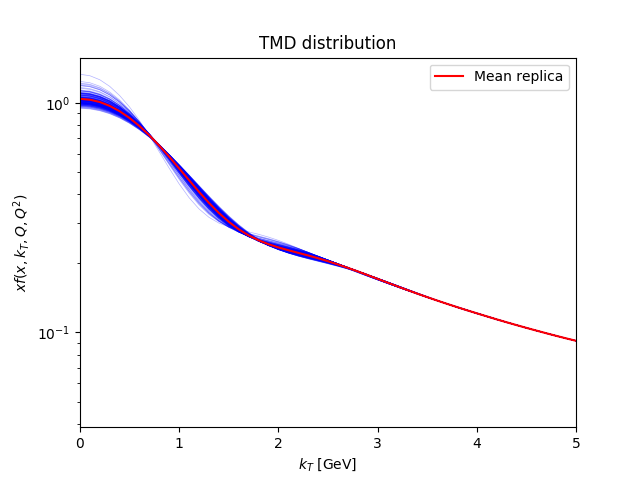
\includegraphics{pngplots/tmd_1_2_0.001.png}
\caption{TMD PDF of the \(d\) at \(Q = 2\) GeV and \(x = 0.001\)}
\end{figure}

\begin{figure}
\centering
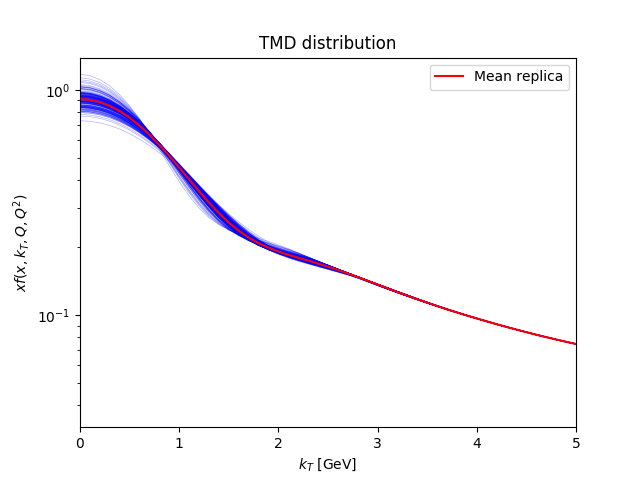
\includegraphics{pngplots/tmd_1_2_0.01.png}
\caption{TMD PDF of the \(d\) at \(Q = 2\) GeV and \(x = 0.01\)}
\end{figure}

\begin{figure}
\centering
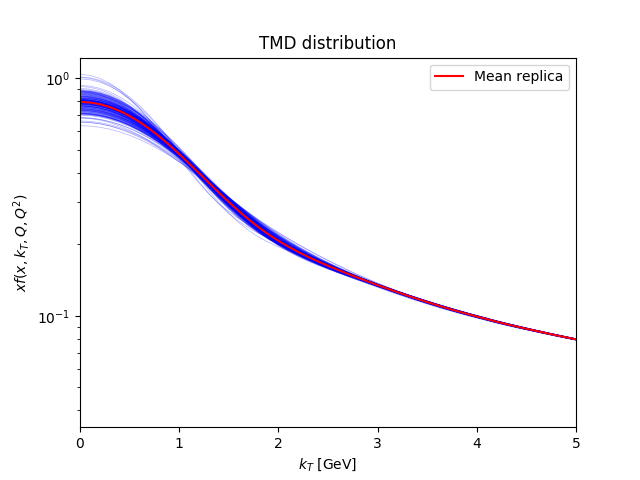
\includegraphics{pngplots/tmd_1_2_0.1.png}
\caption{TMD PDF of the \(d\) at \(Q = 2\) GeV and \(x = 0.1\)}
\end{figure}

\begin{figure}
\centering
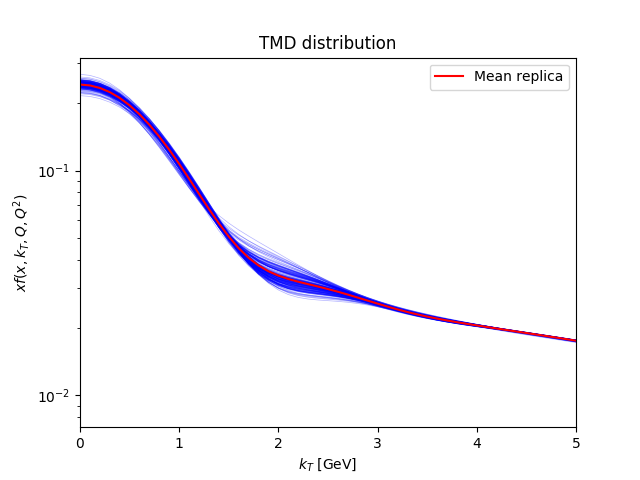
\includegraphics{pngplots/tmd_1_2_0.5.png}
\caption{TMD PDF of the \(d\) at \(Q = 2\) GeV and \(x = 0.5\)}
\end{figure}

\begin{figure}
\centering
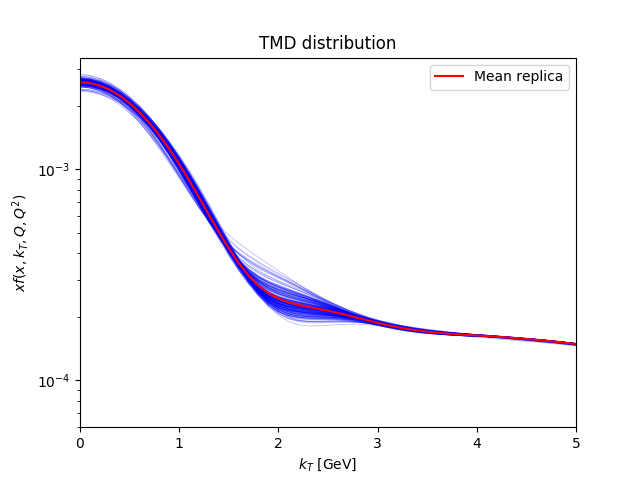
\includegraphics{pngplots/tmd_1_2_0.9.png}
\caption{TMD PDF of the \(d\) at \(Q = 2\) GeV and \(x = 0.9\)}
\end{figure}

\hypertarget{data-theory-comparison}{%
\subsection{Data-theory comparison}\label{data-theory-comparison}}

\begin{figure}
\centering
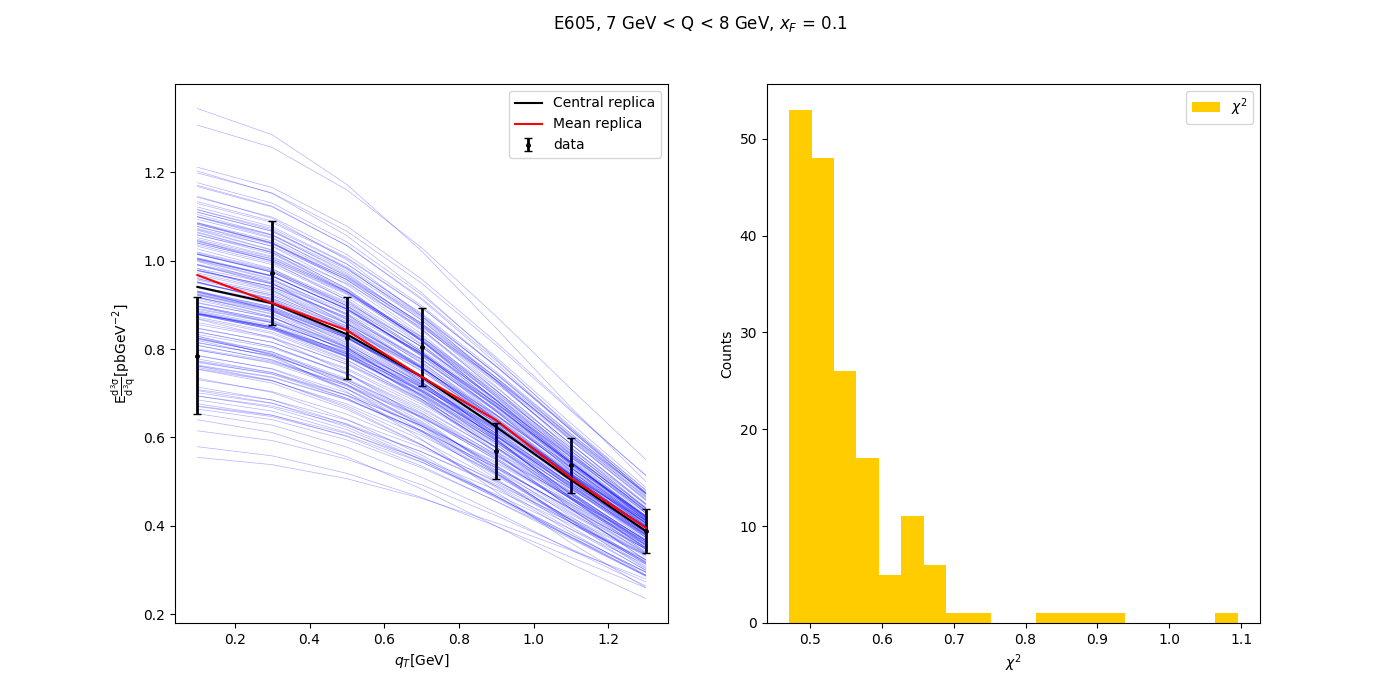
\includegraphics{pngplots/E605_Q_7_8.png}
\caption{E605\_Q\_7\_8 data-theory comparison}
\end{figure}

\begin{figure}
\centering
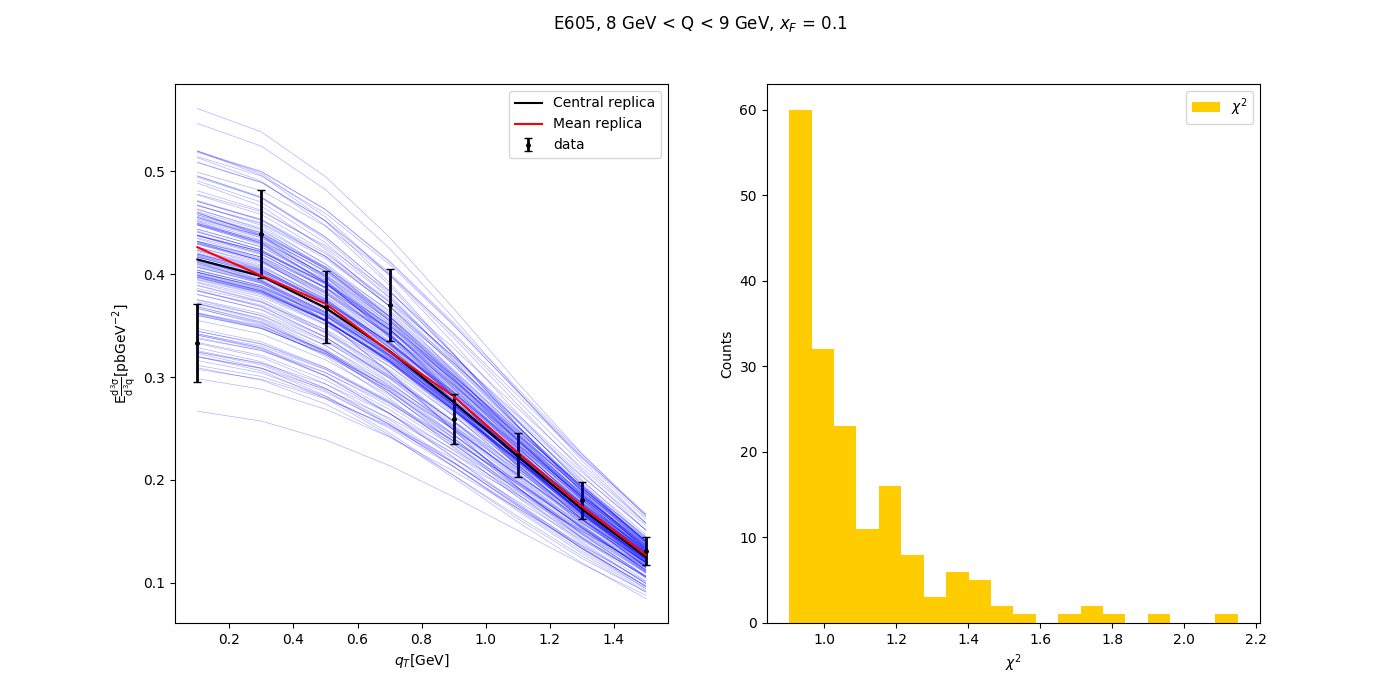
\includegraphics{pngplots/E605_Q_8_9.png}
\caption{E605\_Q\_8\_9 data-theory comparison}
\end{figure}

\begin{figure}
\centering
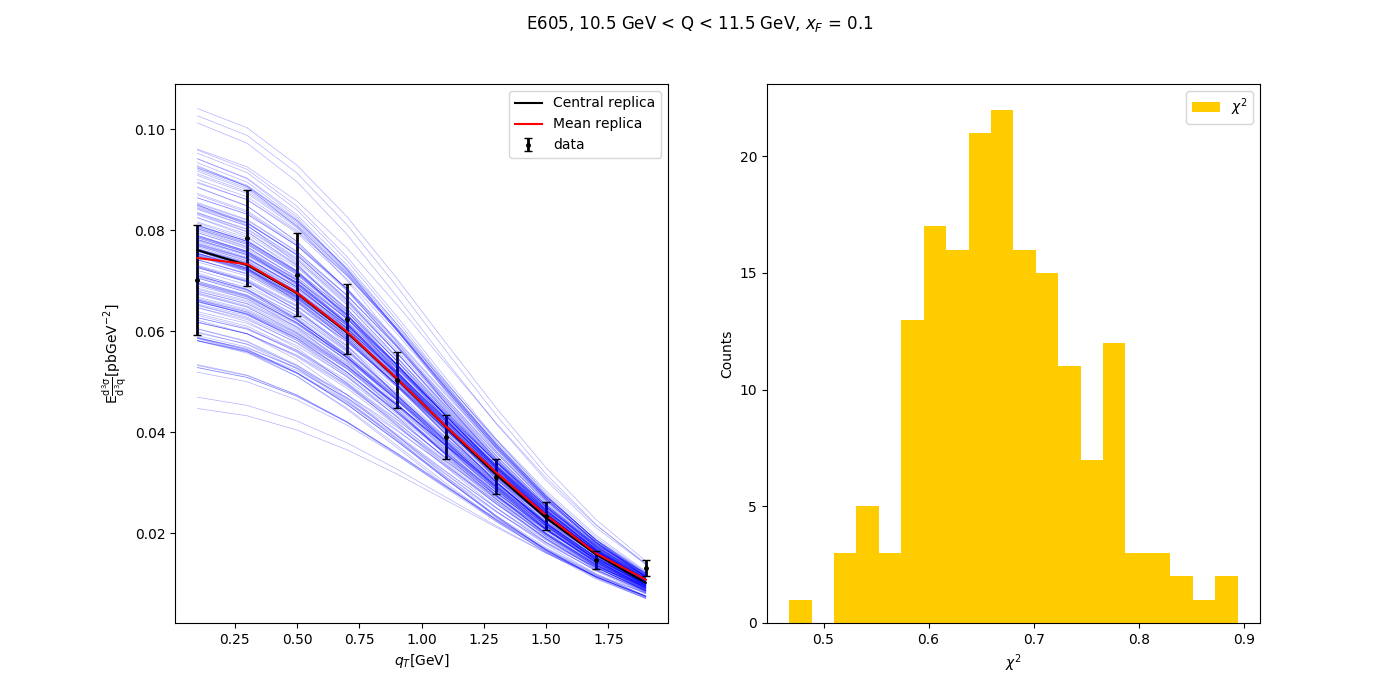
\includegraphics{pngplots/E605_Q_10.5_11.5.png}
\caption{E605\_Q\_10.5\_11.5 data-theory comparison}
\end{figure}

\begin{figure}
\centering
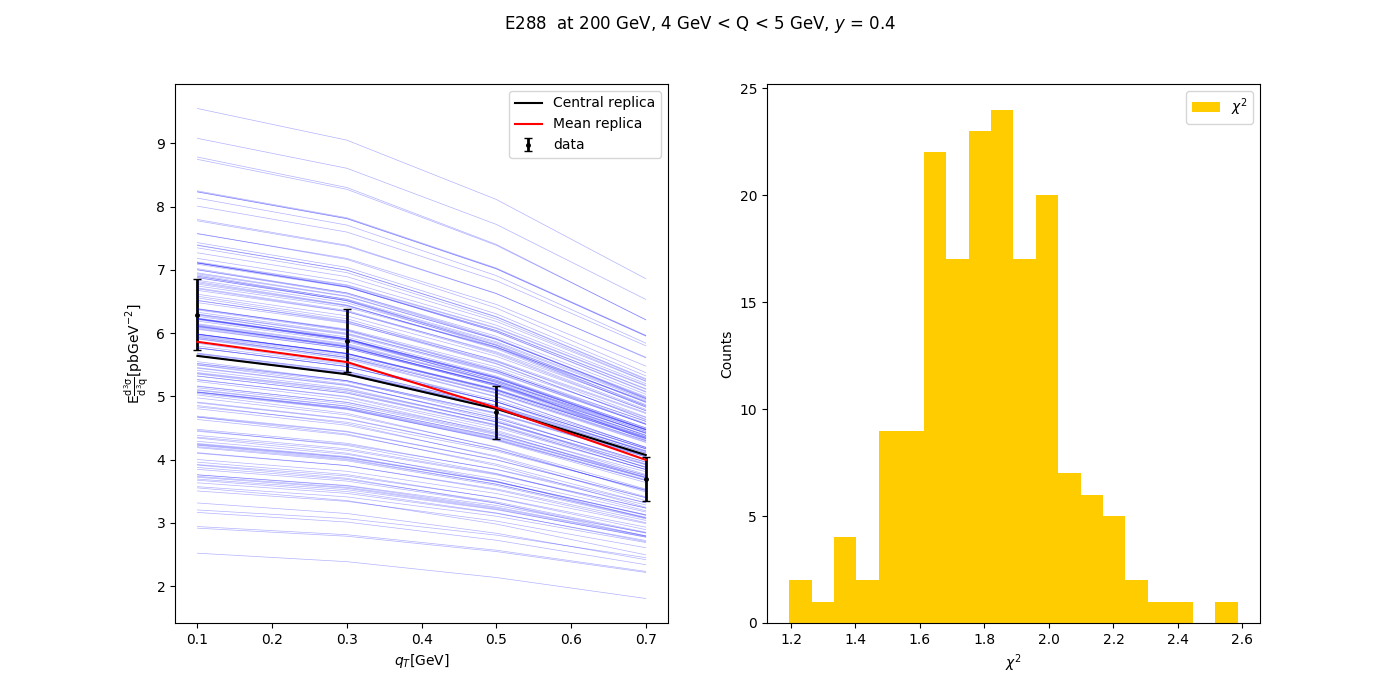
\includegraphics{pngplots/E288_200_Q_4_5.png}
\caption{E288\_200\_Q\_4\_5 data-theory comparison}
\end{figure}

\begin{figure}
\centering
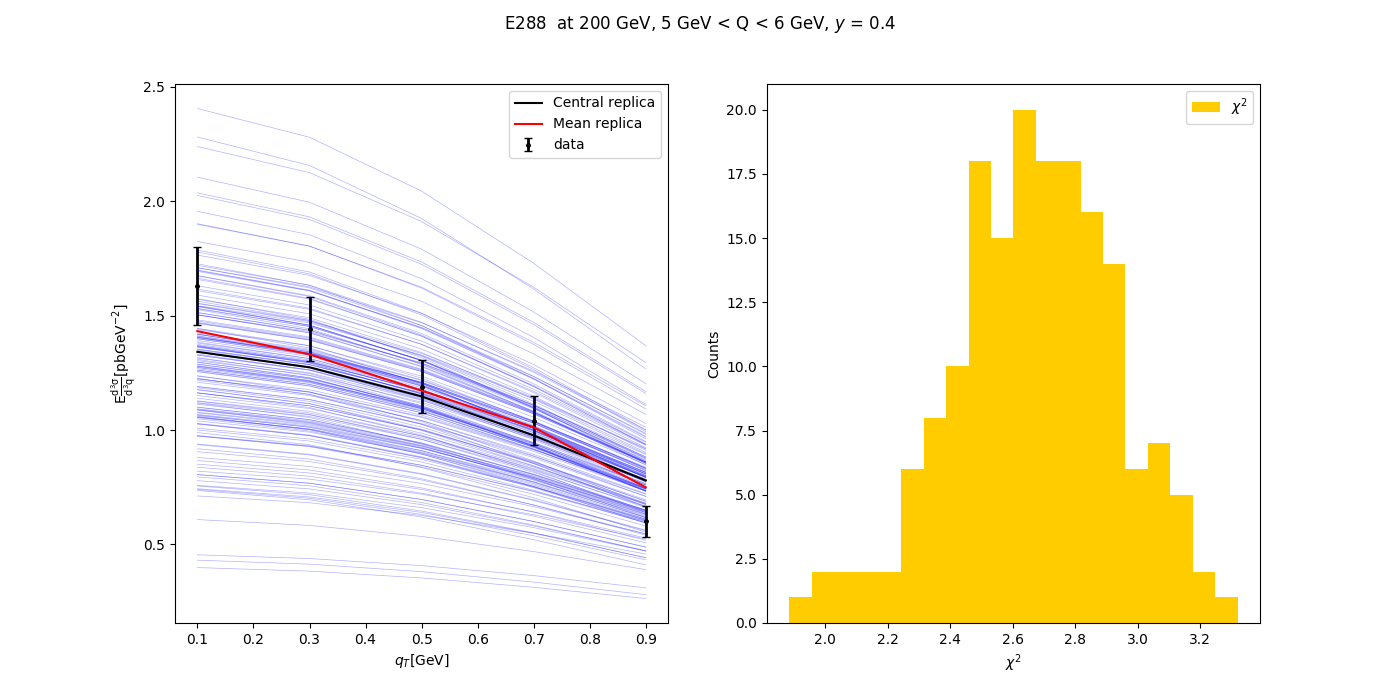
\includegraphics{pngplots/E288_200_Q_5_6.png}
\caption{E288\_200\_Q\_5\_6 data-theory comparison}
\end{figure}

\begin{figure}
\centering
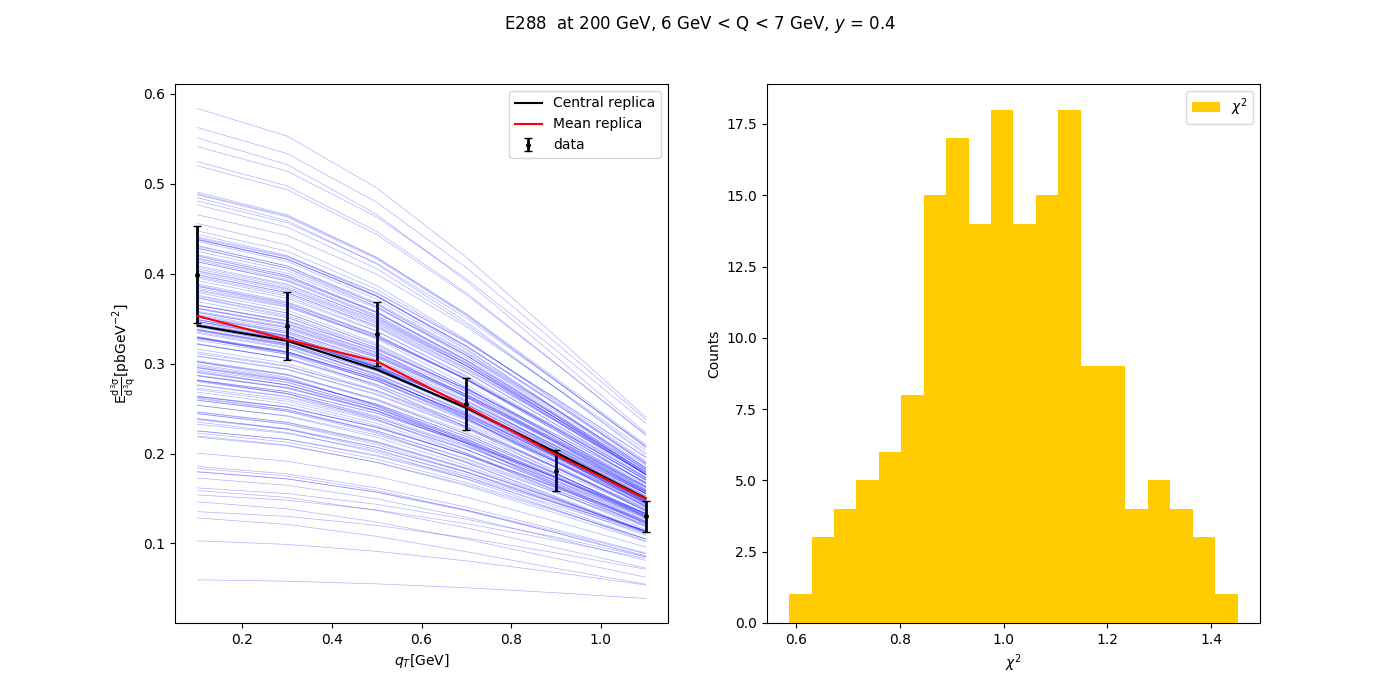
\includegraphics{pngplots/E288_200_Q_6_7.png}
\caption{E288\_200\_Q\_6\_7 data-theory comparison}
\end{figure}

\begin{figure}
\centering
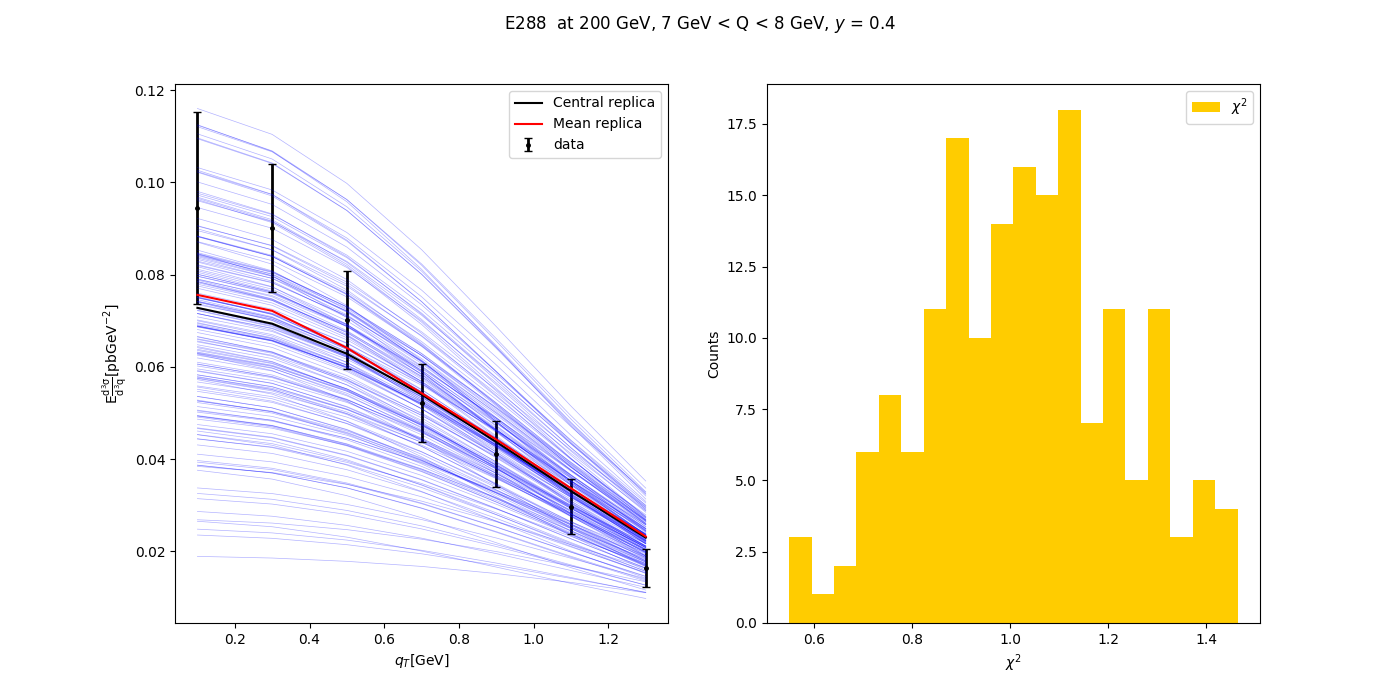
\includegraphics{pngplots/E288_200_Q_7_8.png}
\caption{E288\_200\_Q\_7\_8 data-theory comparison}
\end{figure}

\begin{figure}
\centering
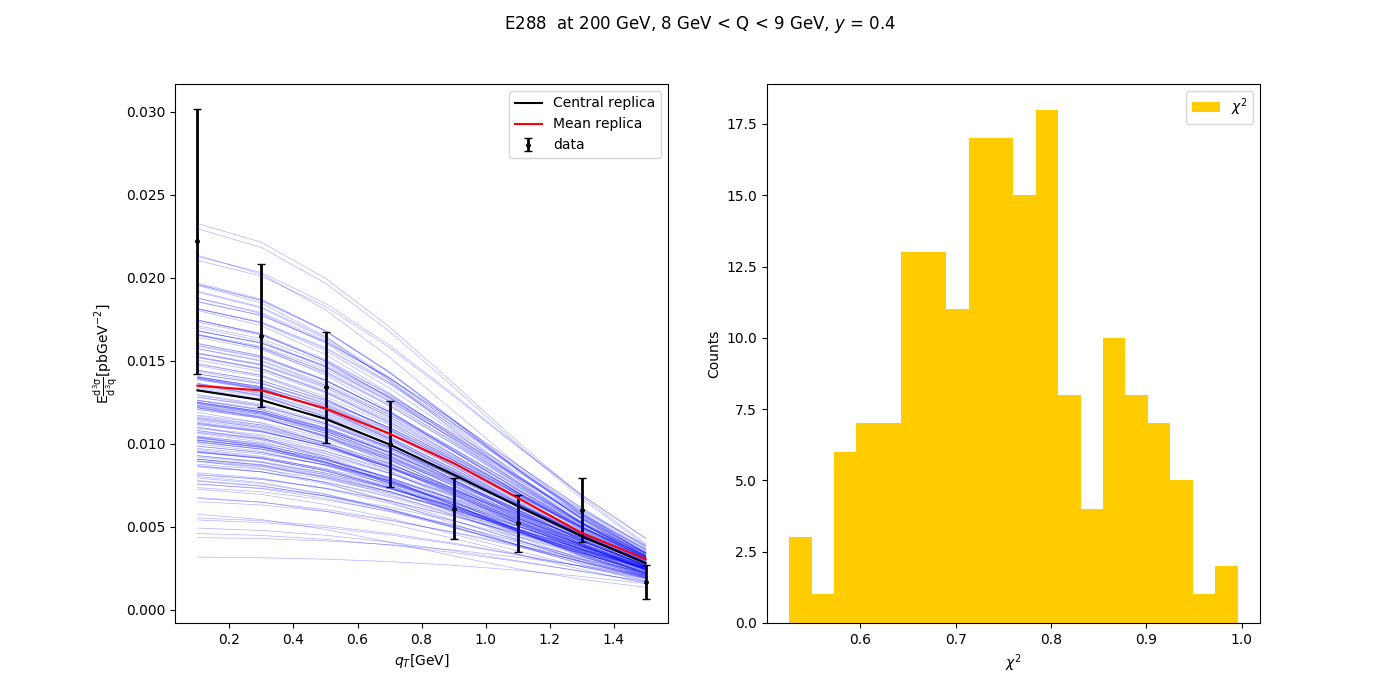
\includegraphics{pngplots/E288_200_Q_8_9.png}
\caption{E288\_200\_Q\_8\_9 data-theory comparison}
\end{figure}

\begin{figure}
\centering
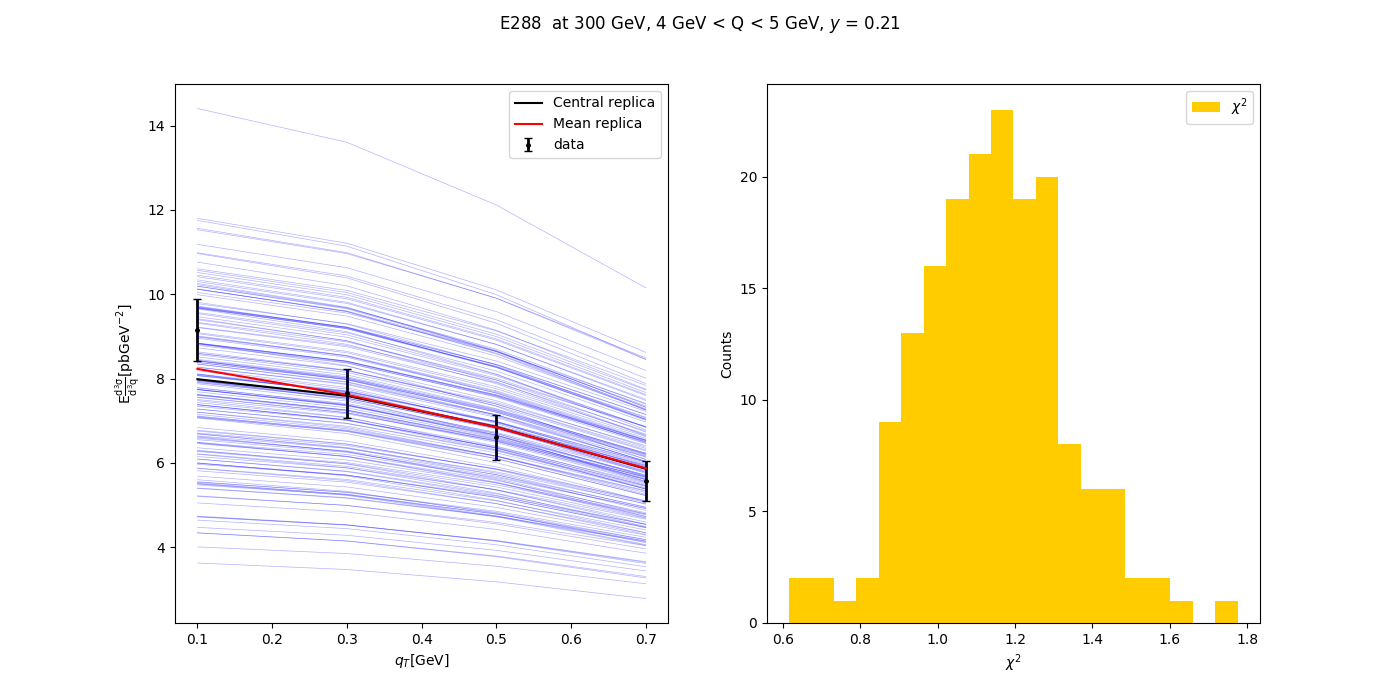
\includegraphics{pngplots/E288_300_Q_4_5.png}
\caption{E288\_300\_Q\_4\_5 data-theory comparison}
\end{figure}

\begin{figure}
\centering
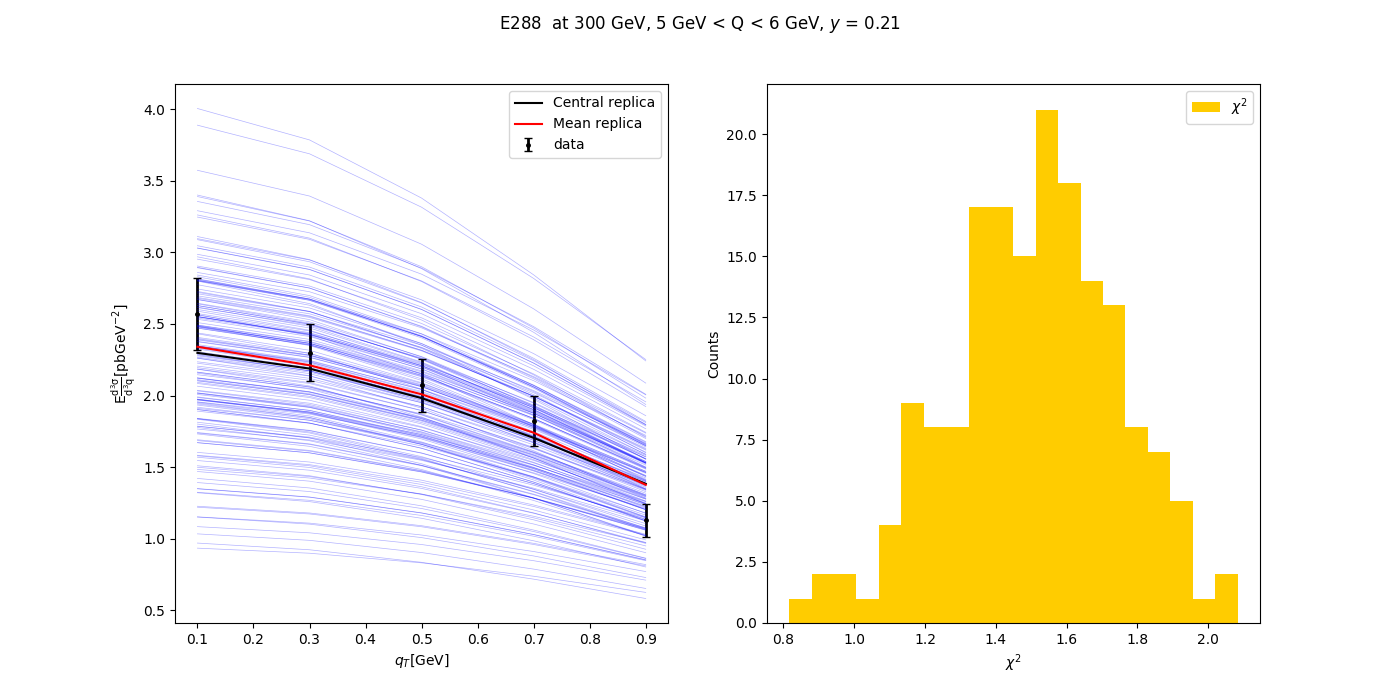
\includegraphics{pngplots/E288_300_Q_5_6.png}
\caption{E288\_300\_Q\_5\_6 data-theory comparison}
\end{figure}

\begin{figure}
\centering
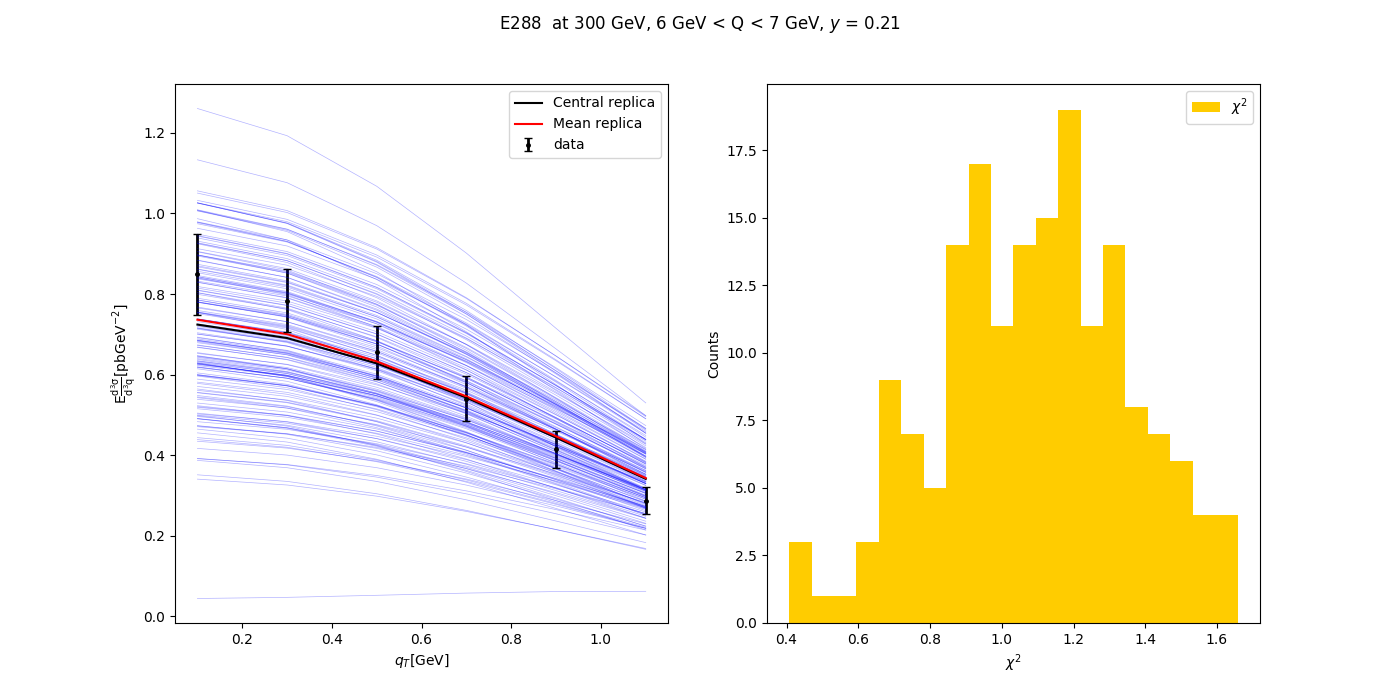
\includegraphics{pngplots/E288_300_Q_6_7.png}
\caption{E288\_300\_Q\_6\_7 data-theory comparison}
\end{figure}

\begin{figure}
\centering
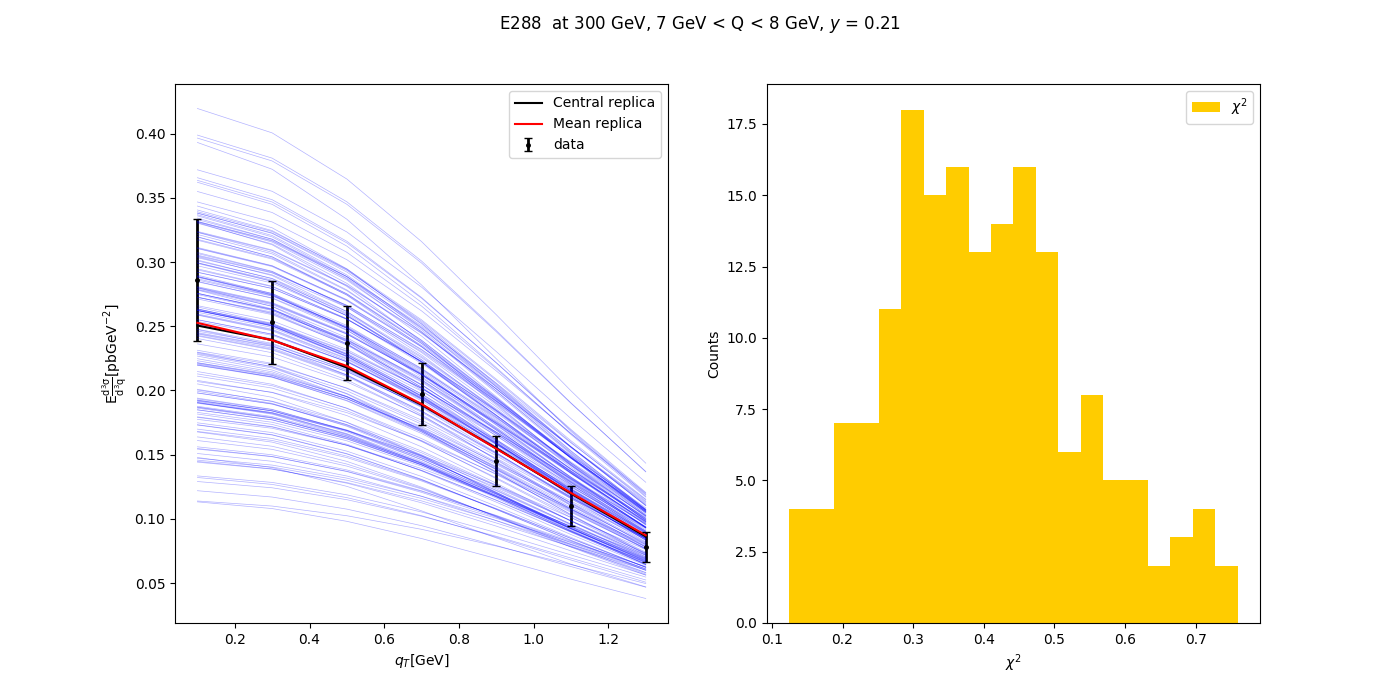
\includegraphics{pngplots/E288_300_Q_7_8.png}
\caption{E288\_300\_Q\_7\_8 data-theory comparison}
\end{figure}

\begin{figure}
\centering
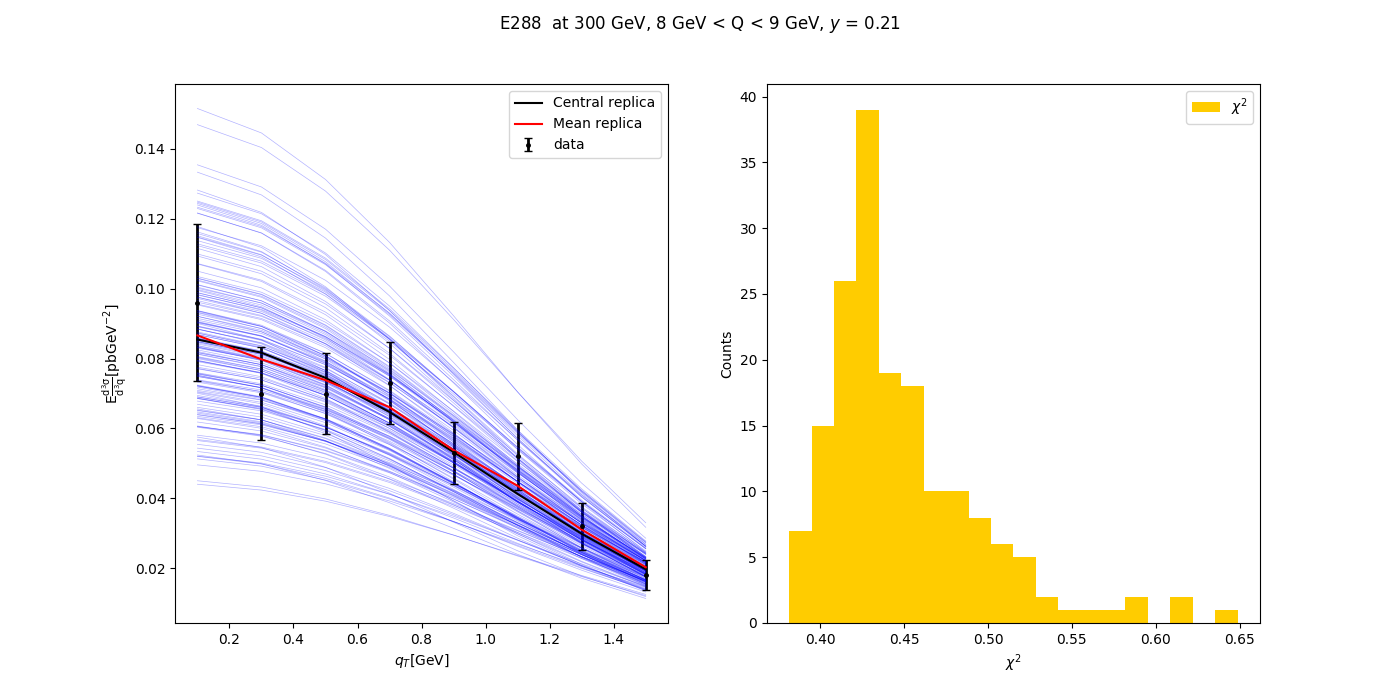
\includegraphics{pngplots/E288_300_Q_8_9.png}
\caption{E288\_300\_Q\_8\_9 data-theory comparison}
\end{figure}

\begin{figure}
\centering
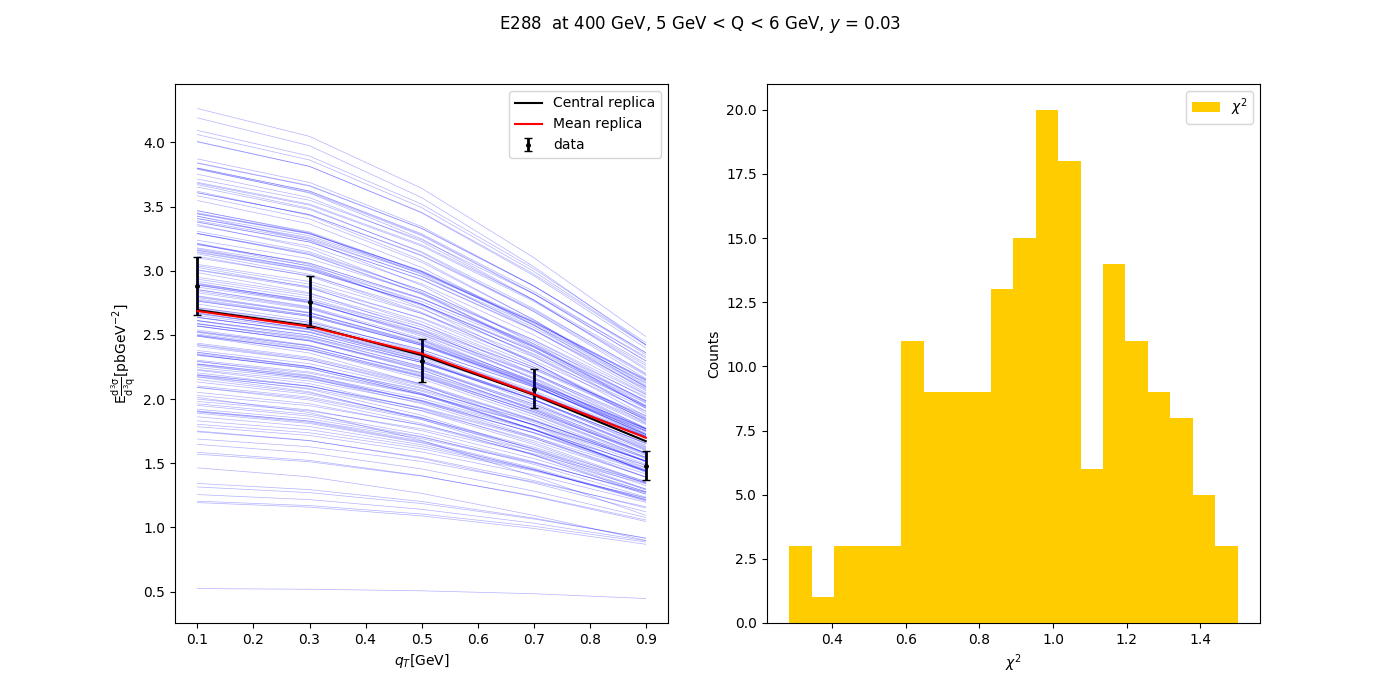
\includegraphics{pngplots/E288_400_Q_5_6.png}
\caption{E288\_400\_Q\_5\_6 data-theory comparison}
\end{figure}

\begin{figure}
\centering
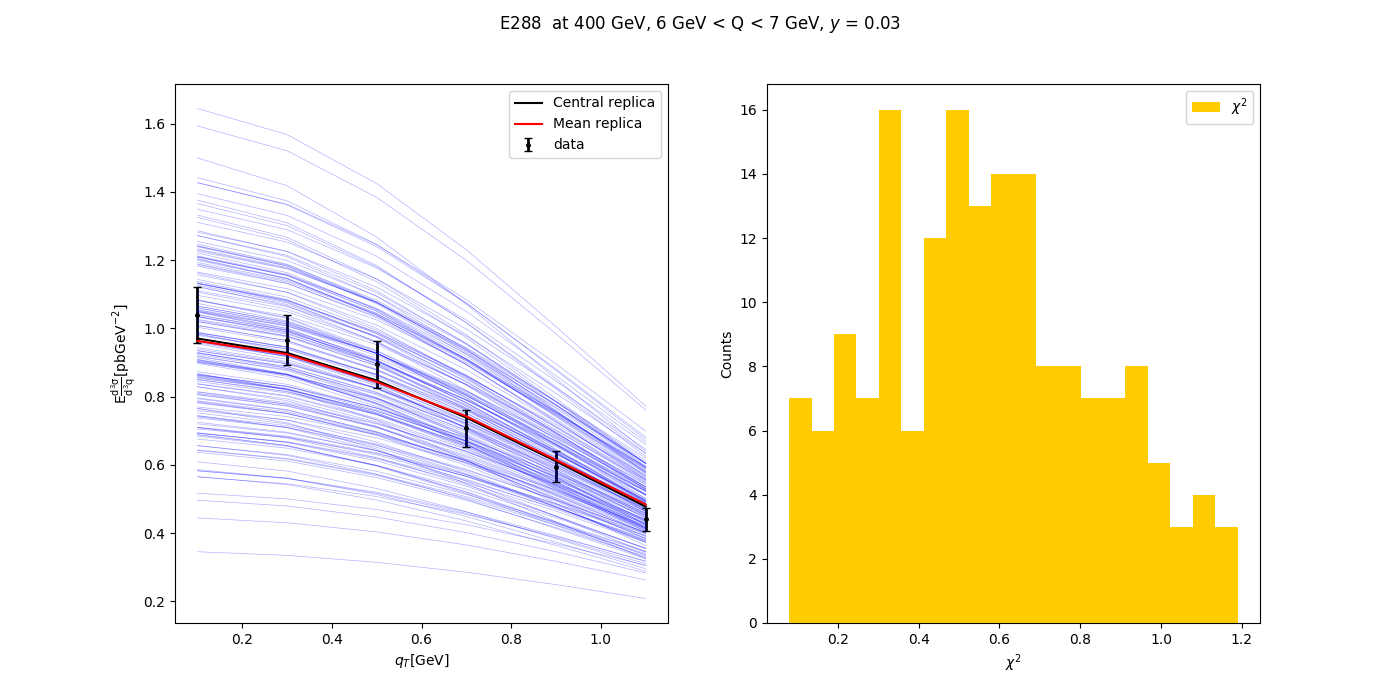
\includegraphics{pngplots/E288_400_Q_6_7.png}
\caption{E288\_400\_Q\_6\_7 data-theory comparison}
\end{figure}

\begin{figure}
\centering
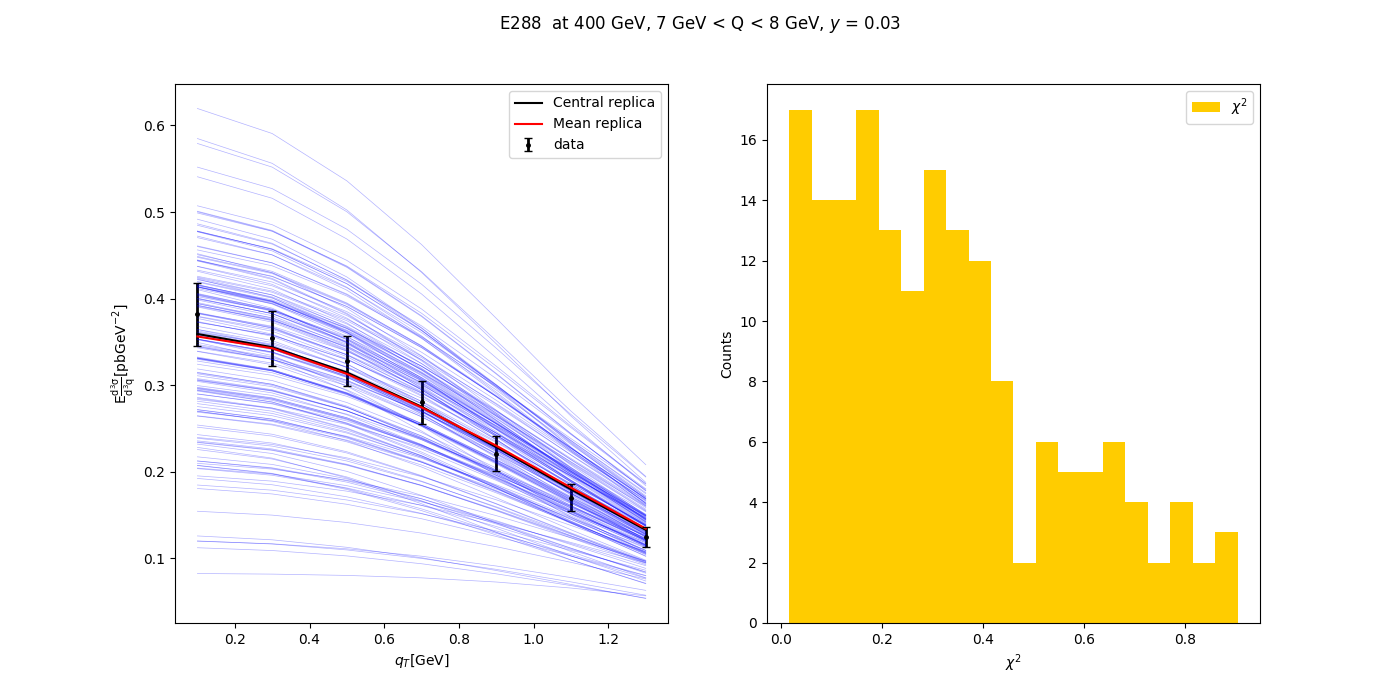
\includegraphics{pngplots/E288_400_Q_7_8.png}
\caption{E288\_400\_Q\_7\_8 data-theory comparison}
\end{figure}

\begin{figure}
\centering
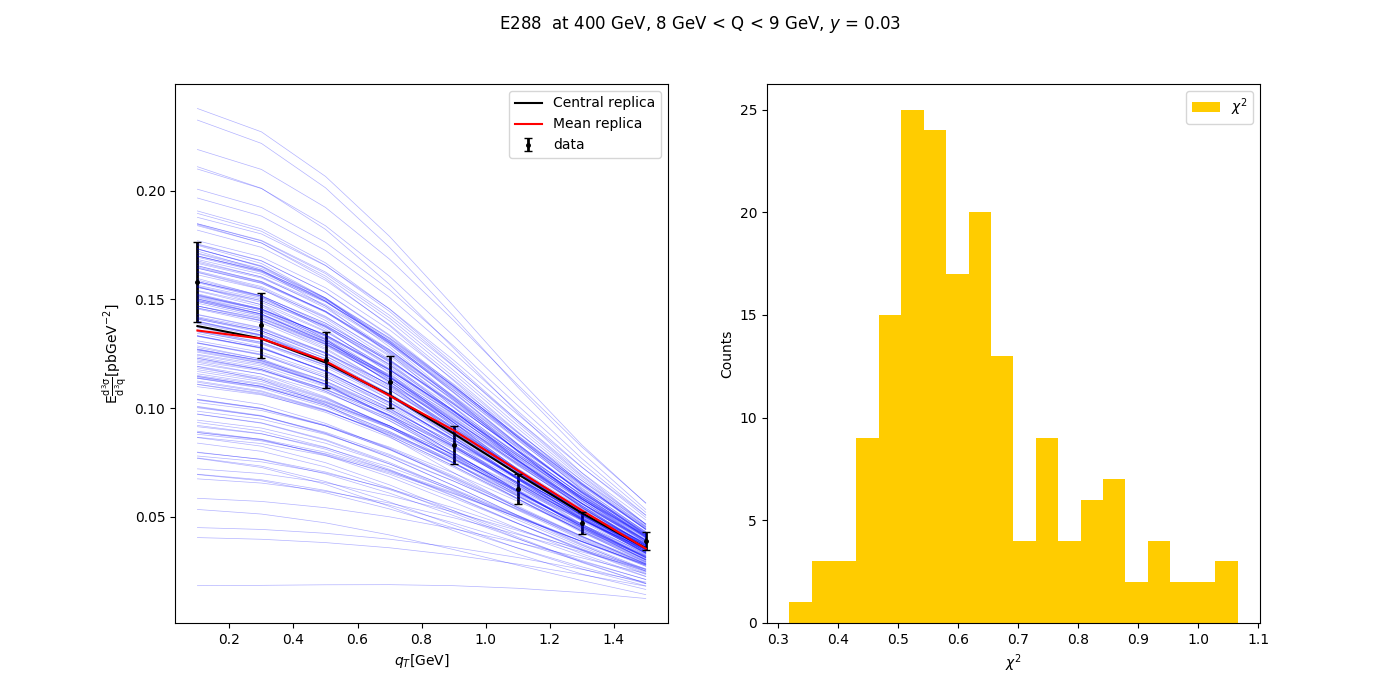
\includegraphics{pngplots/E288_400_Q_8_9.png}
\caption{E288\_400\_Q\_8\_9 data-theory comparison}
\end{figure}

\begin{figure}
\centering
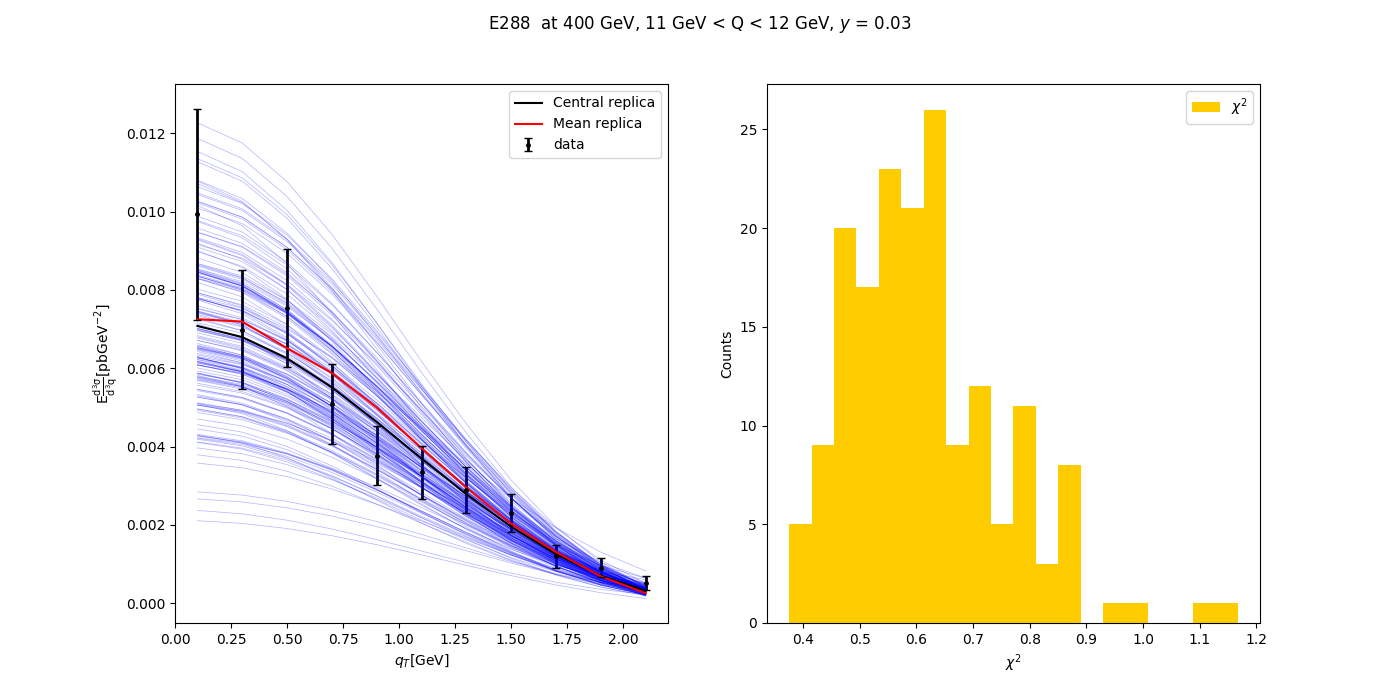
\includegraphics{pngplots/E288_400_Q_11_12.png}
\caption{E288\_400\_Q\_11\_12 data-theory comparison}
\end{figure}

\begin{figure}
\centering
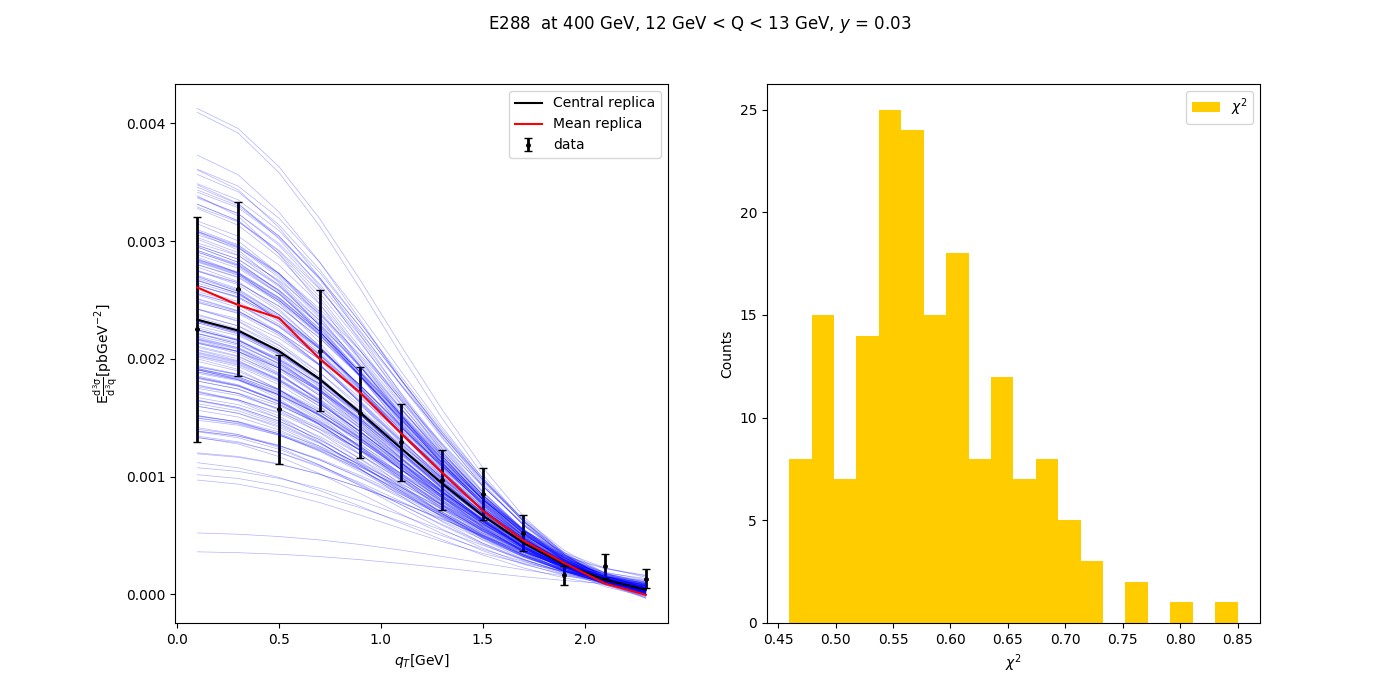
\includegraphics{pngplots/E288_400_Q_12_13.png}
\caption{E288\_400\_Q\_12\_13 data-theory comparison}
\end{figure}

\begin{figure}
\centering
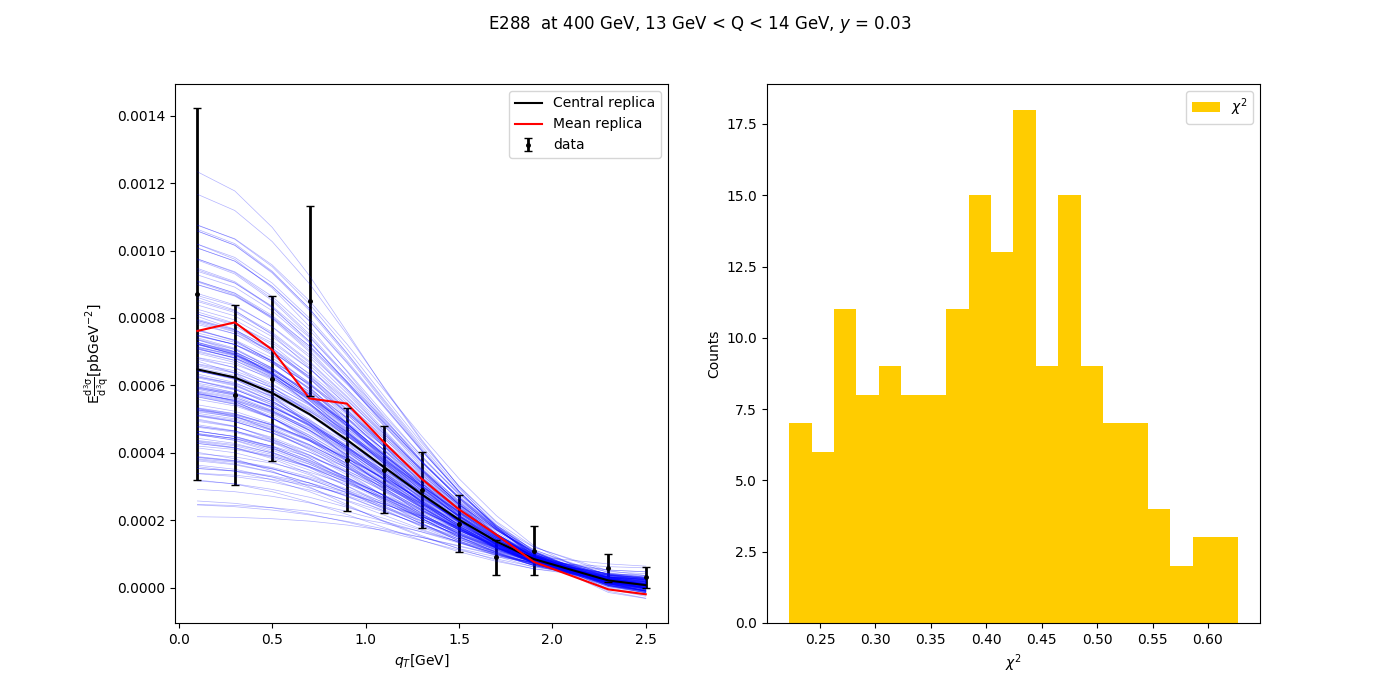
\includegraphics{pngplots/E288_400_Q_13_14.png}
\caption{E288\_400\_Q\_13\_14 data-theory comparison}
\end{figure}

\begin{figure}
\centering
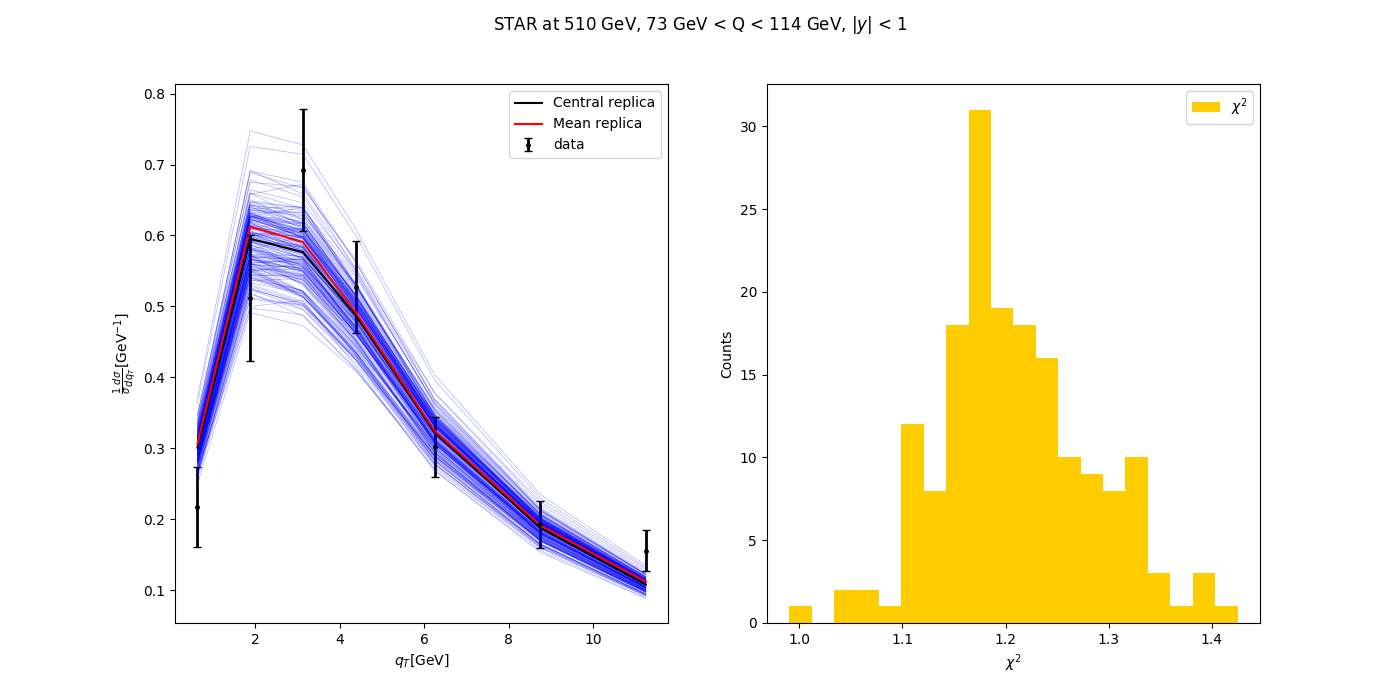
\includegraphics{pngplots/STAR_510.png}
\caption{STAR\_510 data-theory comparison}
\end{figure}

\begin{figure}
\centering
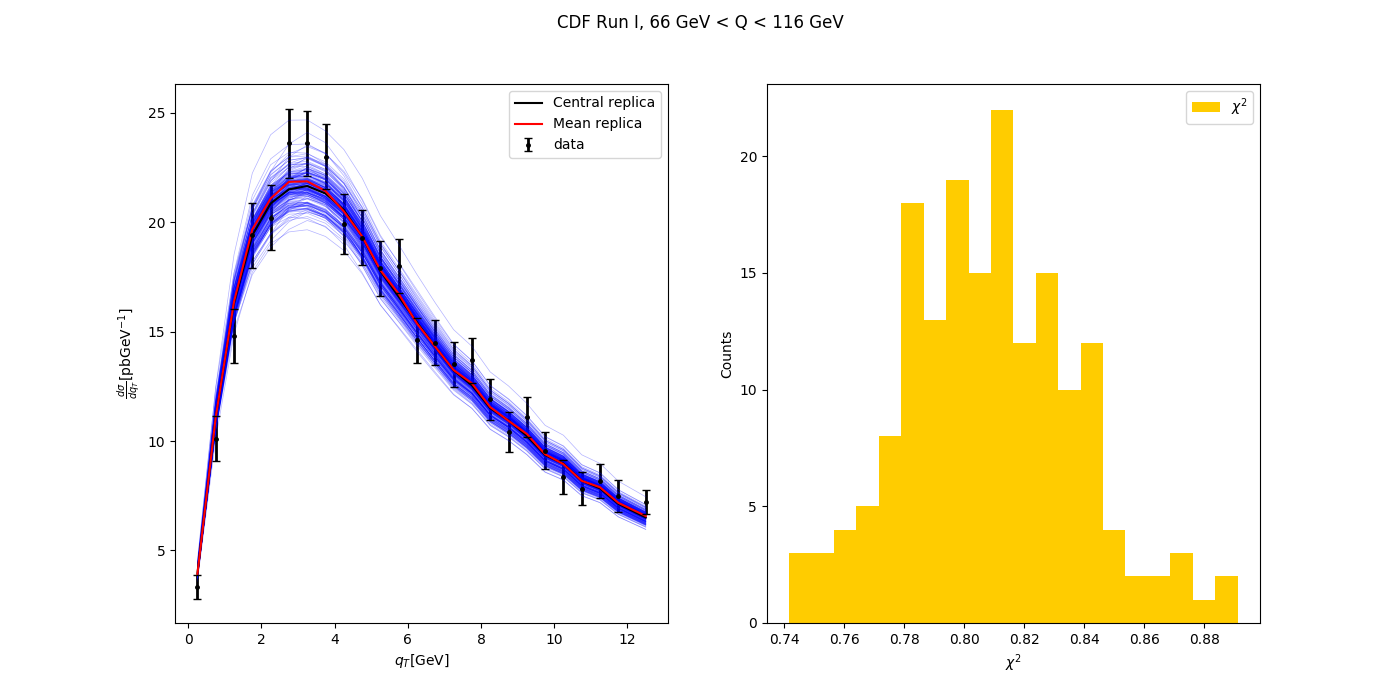
\includegraphics{pngplots/CDF_RunI.png}
\caption{CDF\_RunI data-theory comparison}
\end{figure}

\begin{figure}
\centering
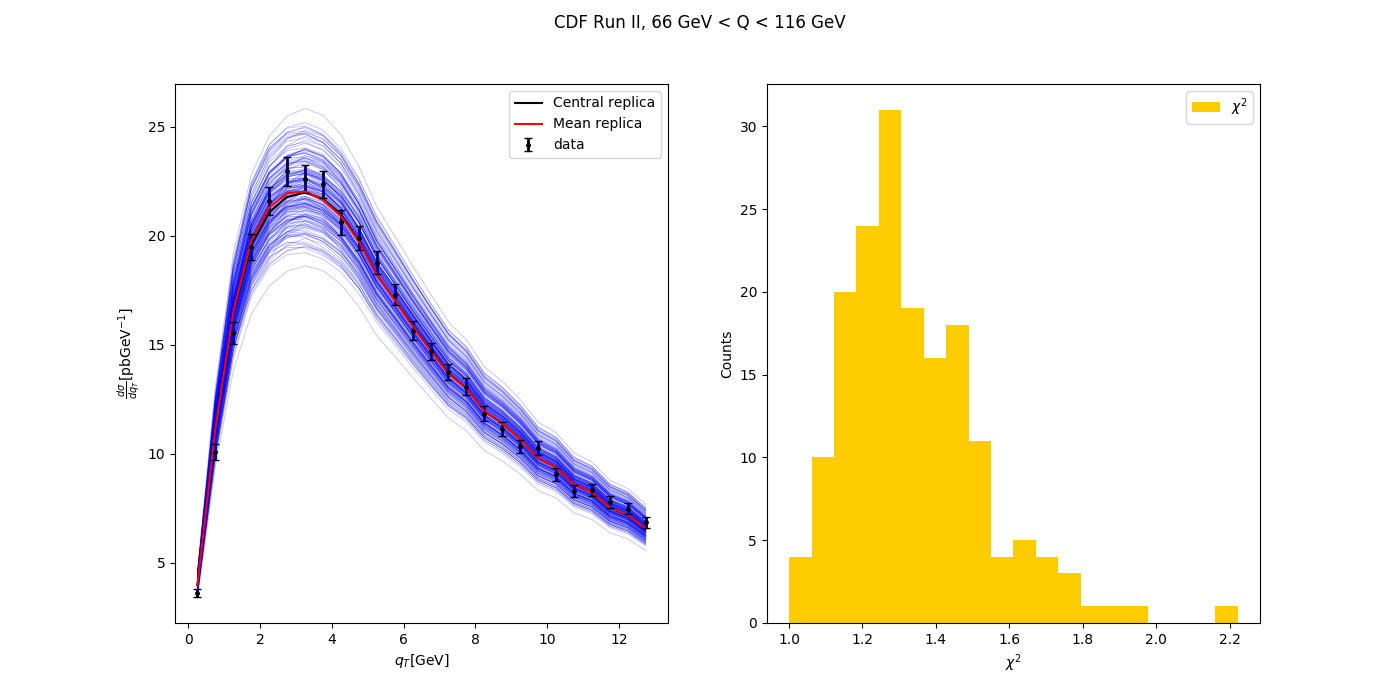
\includegraphics{pngplots/CDF_RunII.png}
\caption{CDF\_RunII data-theory comparison}
\end{figure}

\begin{figure}
\centering
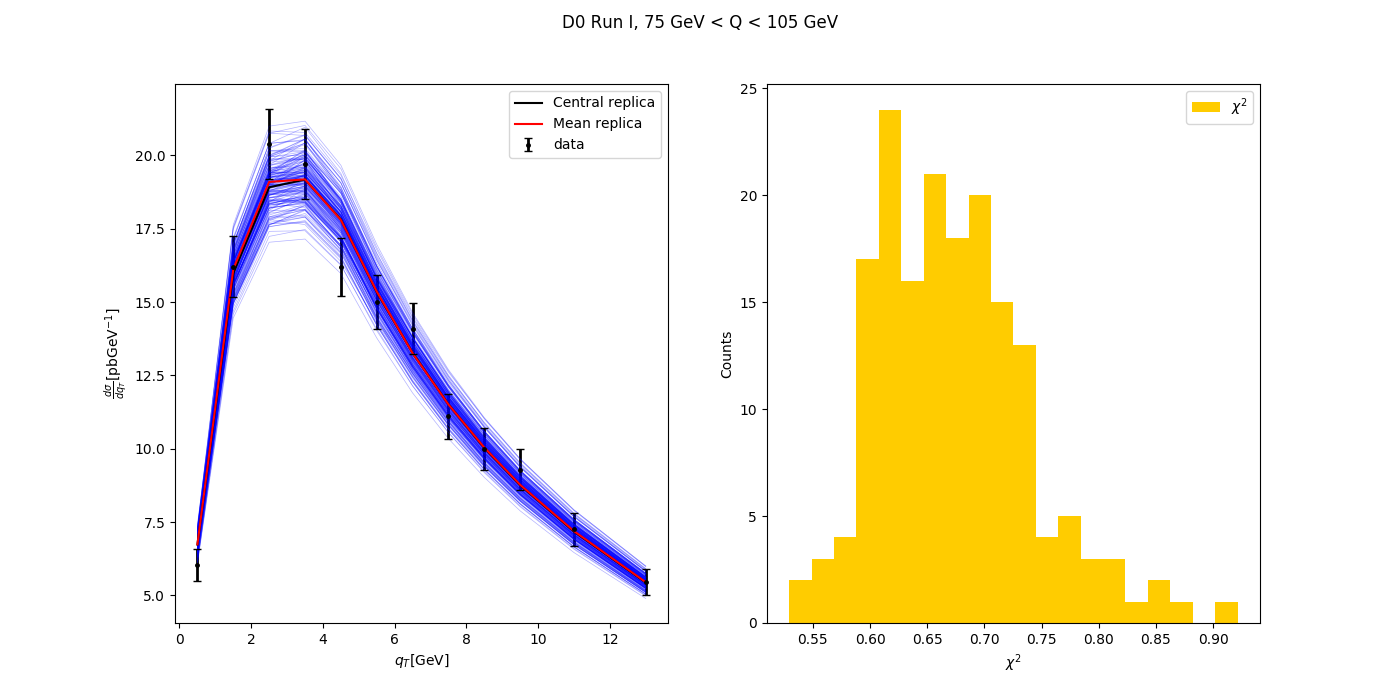
\includegraphics{pngplots/D0_RunI.png}
\caption{D0\_RunI data-theory comparison}
\end{figure}

\begin{figure}
\centering
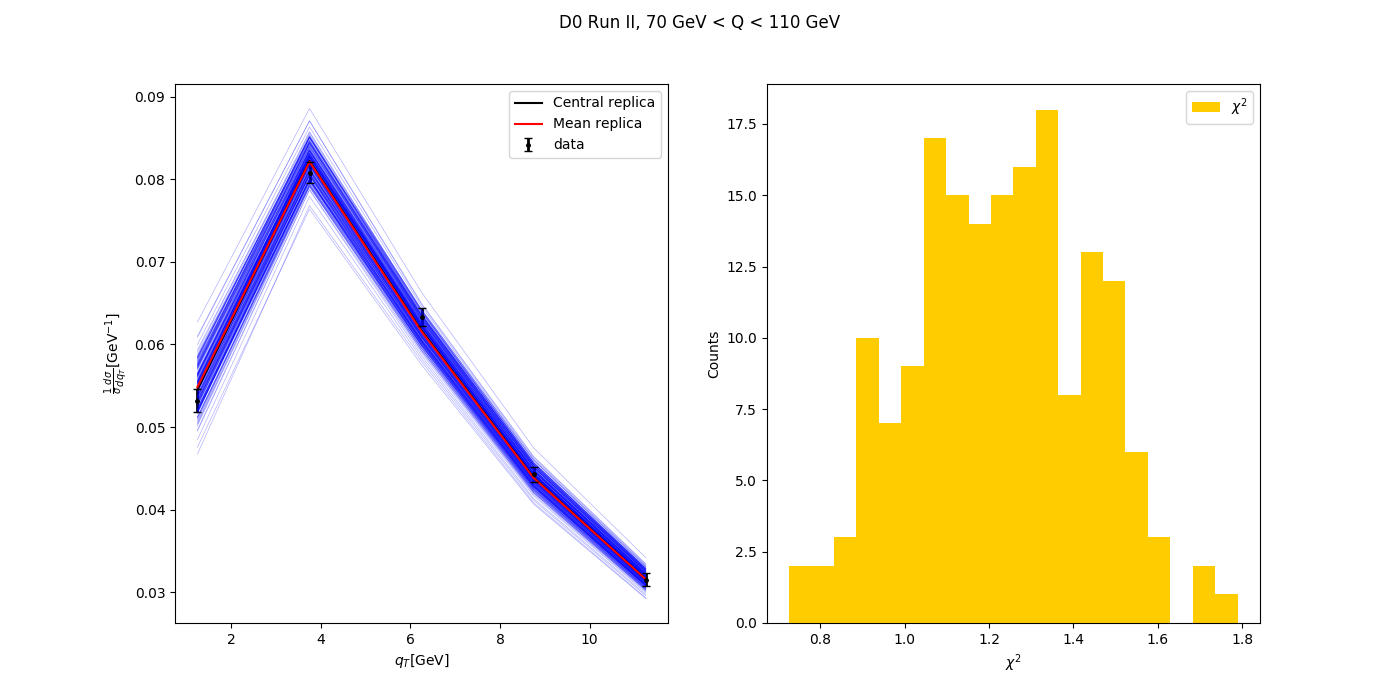
\includegraphics{pngplots/D0_RunII.png}
\caption{D0\_RunII data-theory comparison}
\end{figure}

\begin{figure}
\centering
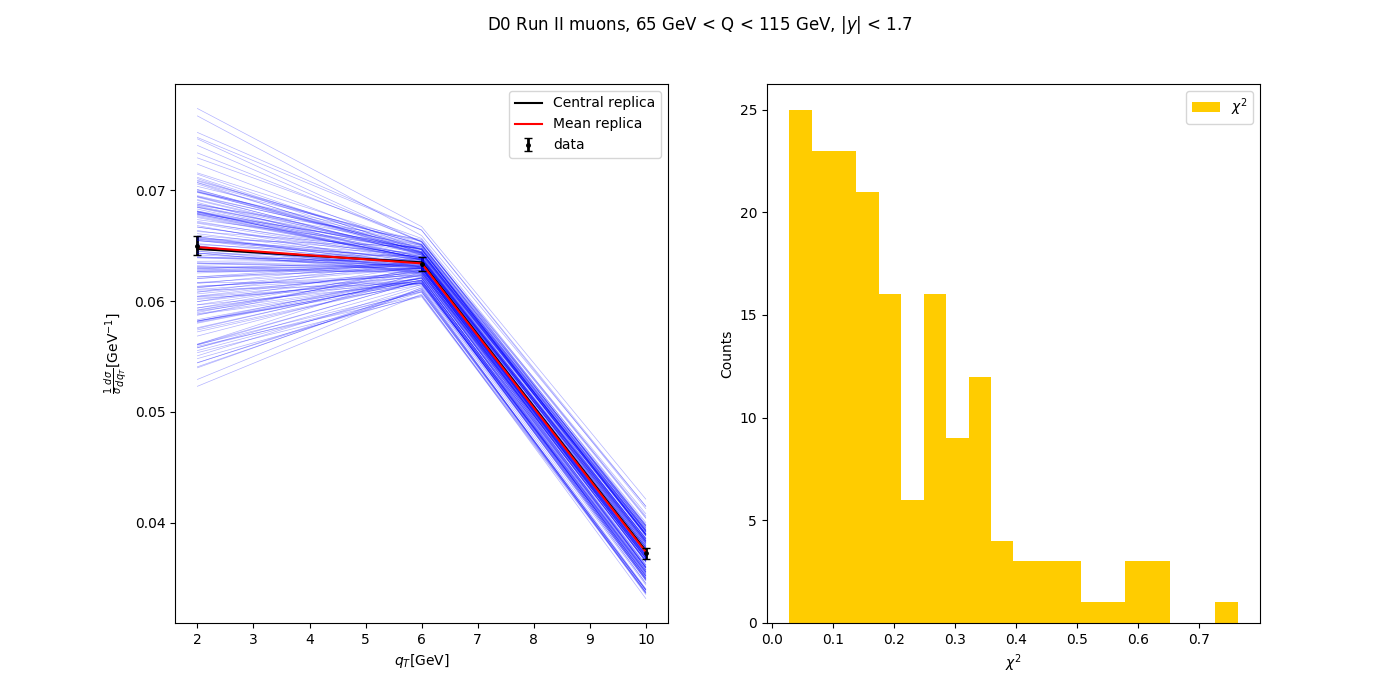
\includegraphics{pngplots/D0_RunIImu.png}
\caption{D0\_RunIImu data-theory comparison}
\end{figure}

\begin{figure}
\centering
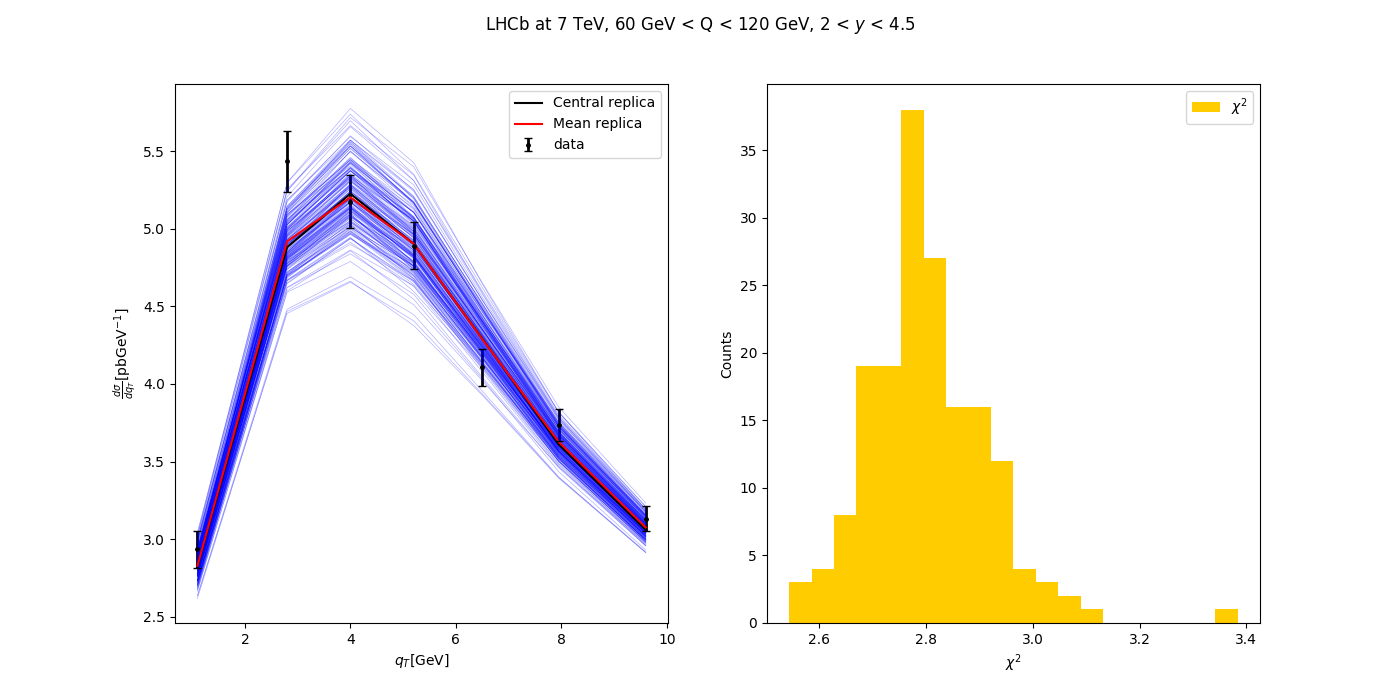
\includegraphics{pngplots/LHCb_7TeV.png}
\caption{LHCb\_7TeV data-theory comparison}
\end{figure}

\begin{figure}
\centering
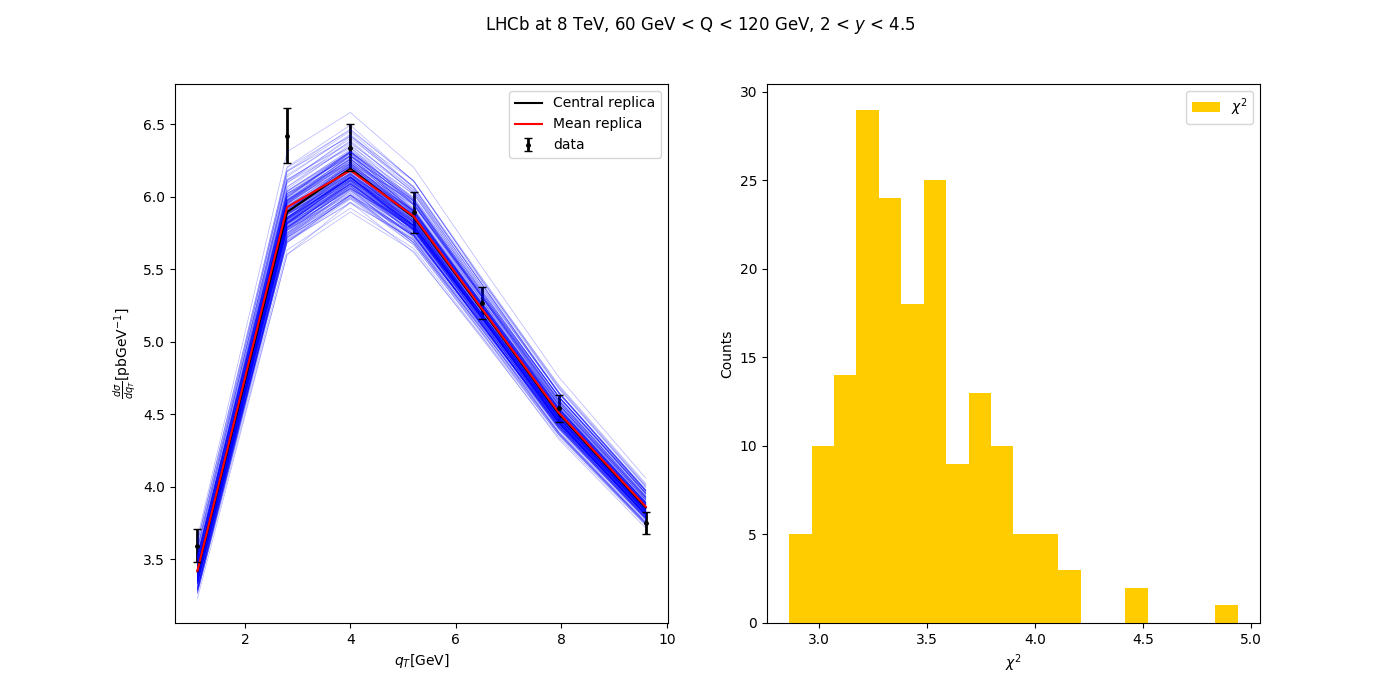
\includegraphics{pngplots/LHCb_8TeV.png}
\caption{LHCb\_8TeV data-theory comparison}
\end{figure}

\begin{figure}
\centering
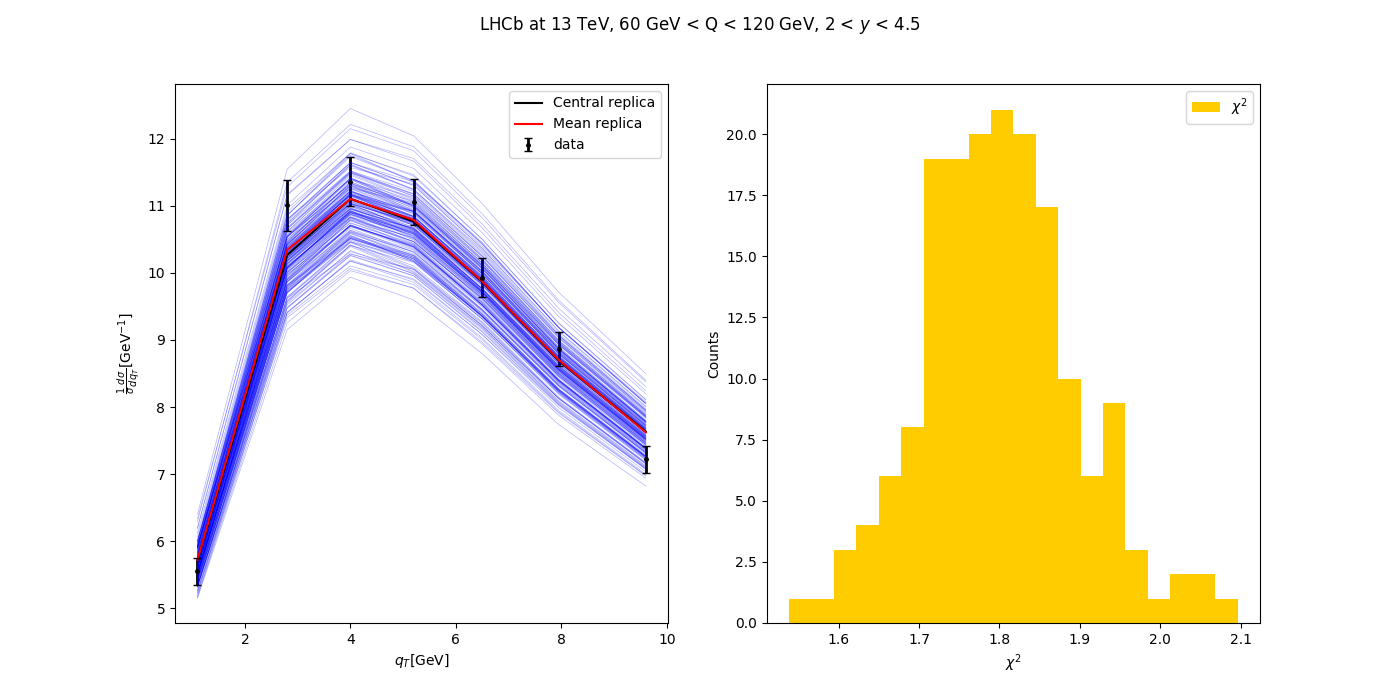
\includegraphics{pngplots/LHCb_13TeV.png}
\caption{LHCb\_13TeV data-theory comparison}
\end{figure}

\begin{figure}
\centering
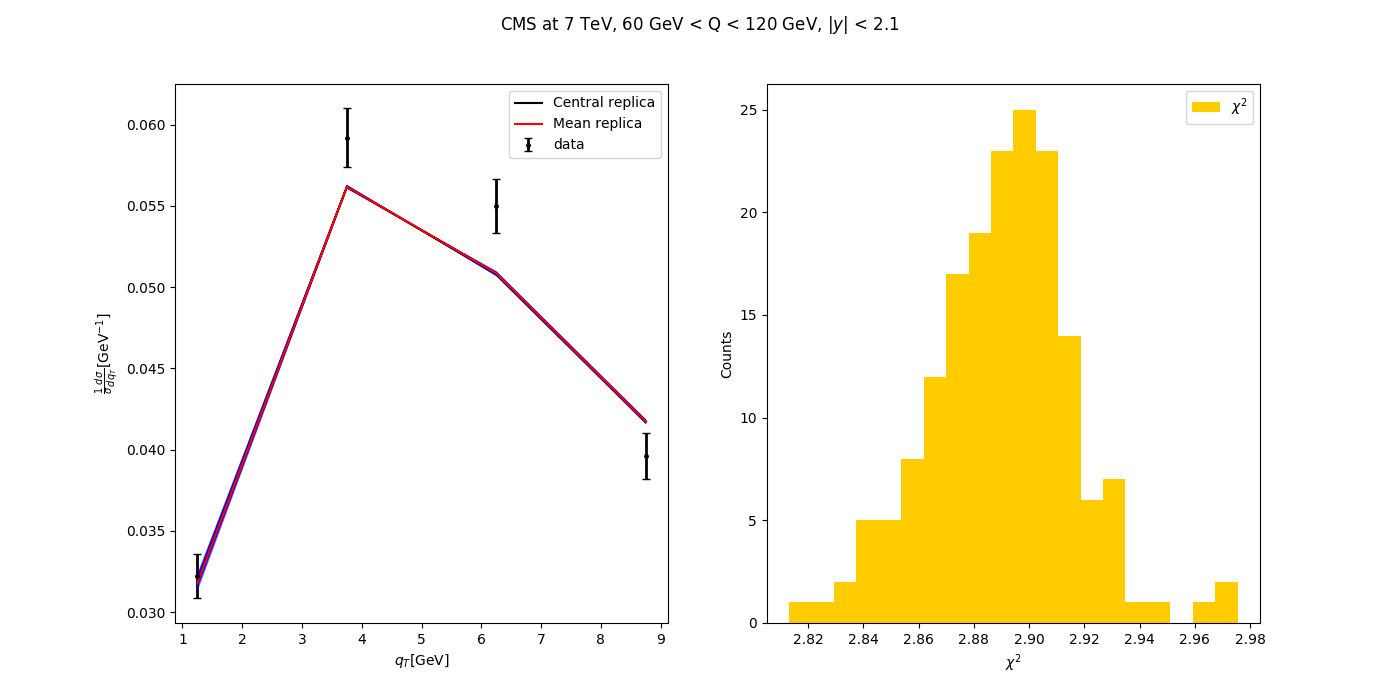
\includegraphics{pngplots/CMS_7TeV.png}
\caption{CMS\_7TeV data-theory comparison}
\end{figure}

\begin{figure}
\centering
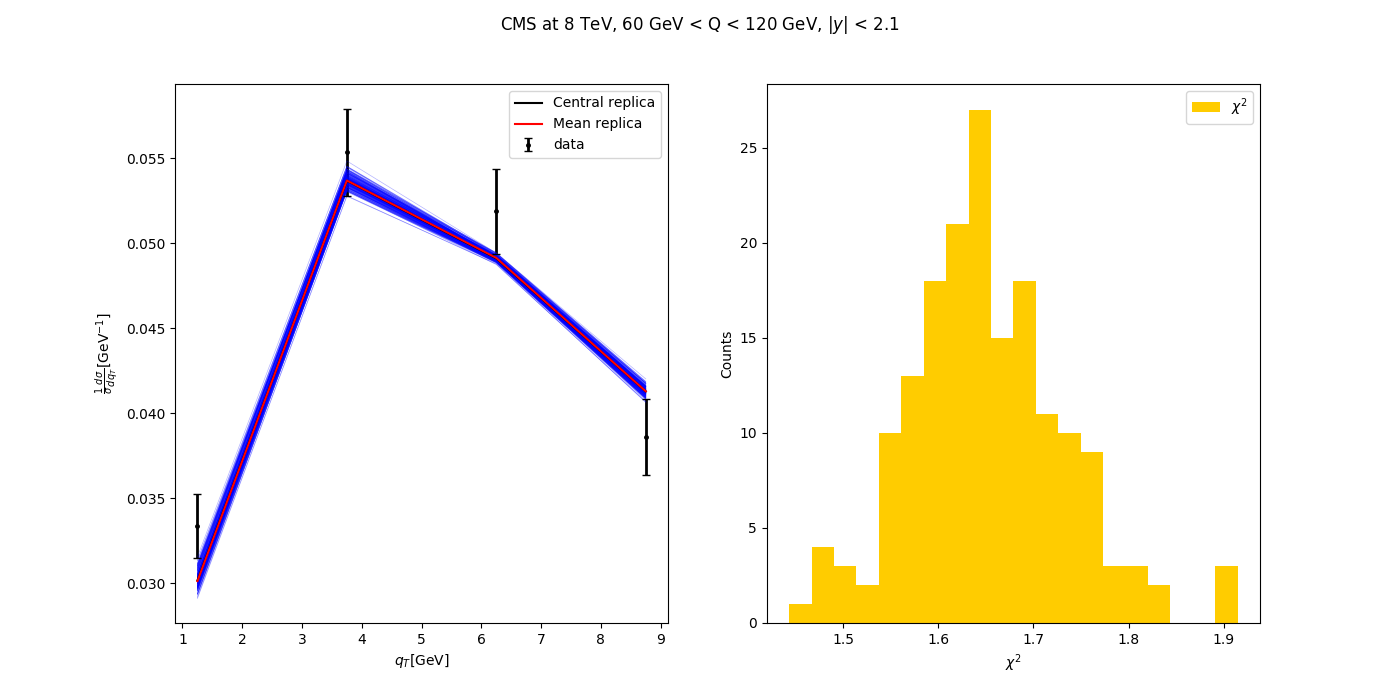
\includegraphics{pngplots/CMS_8TeV.png}
\caption{CMS\_8TeV data-theory comparison}
\end{figure}

\begin{figure}
\centering
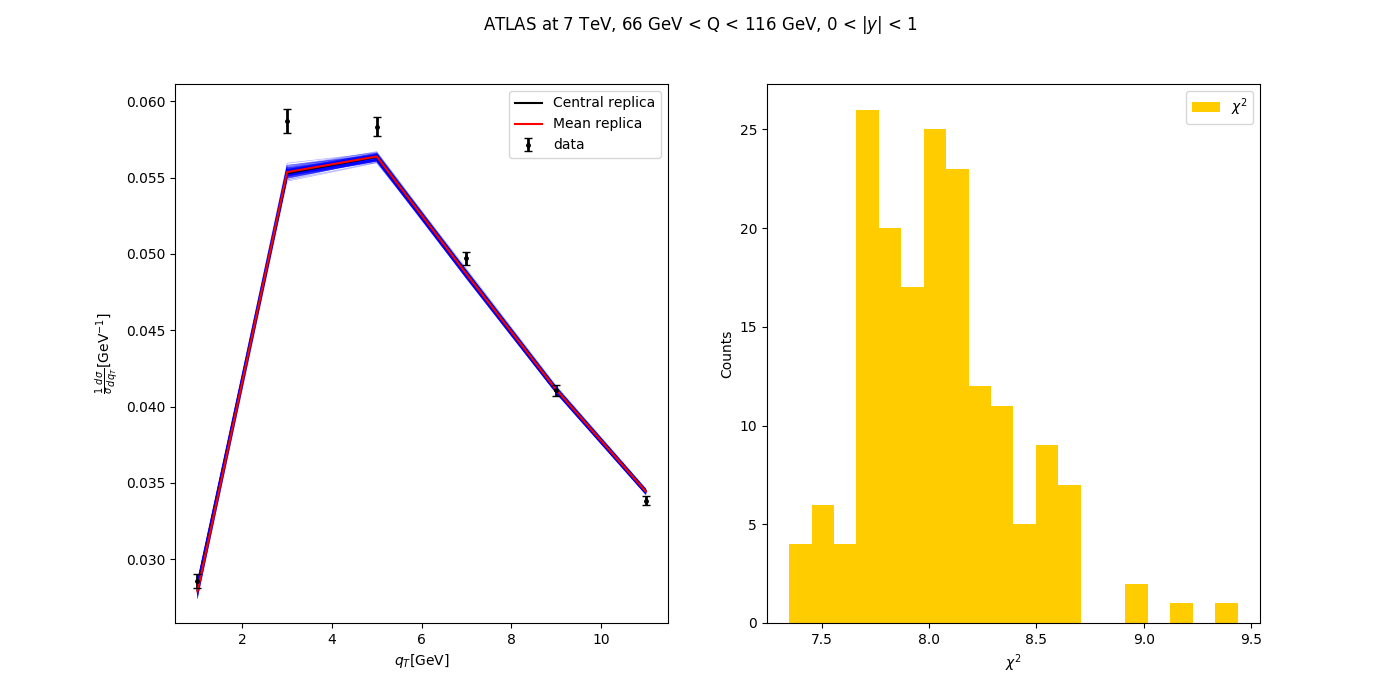
\includegraphics{pngplots/ATLAS_7TeV_y_0_1.png}
\caption{ATLAS\_7TeV\_y\_0\_1 data-theory comparison}
\end{figure}

\begin{figure}
\centering
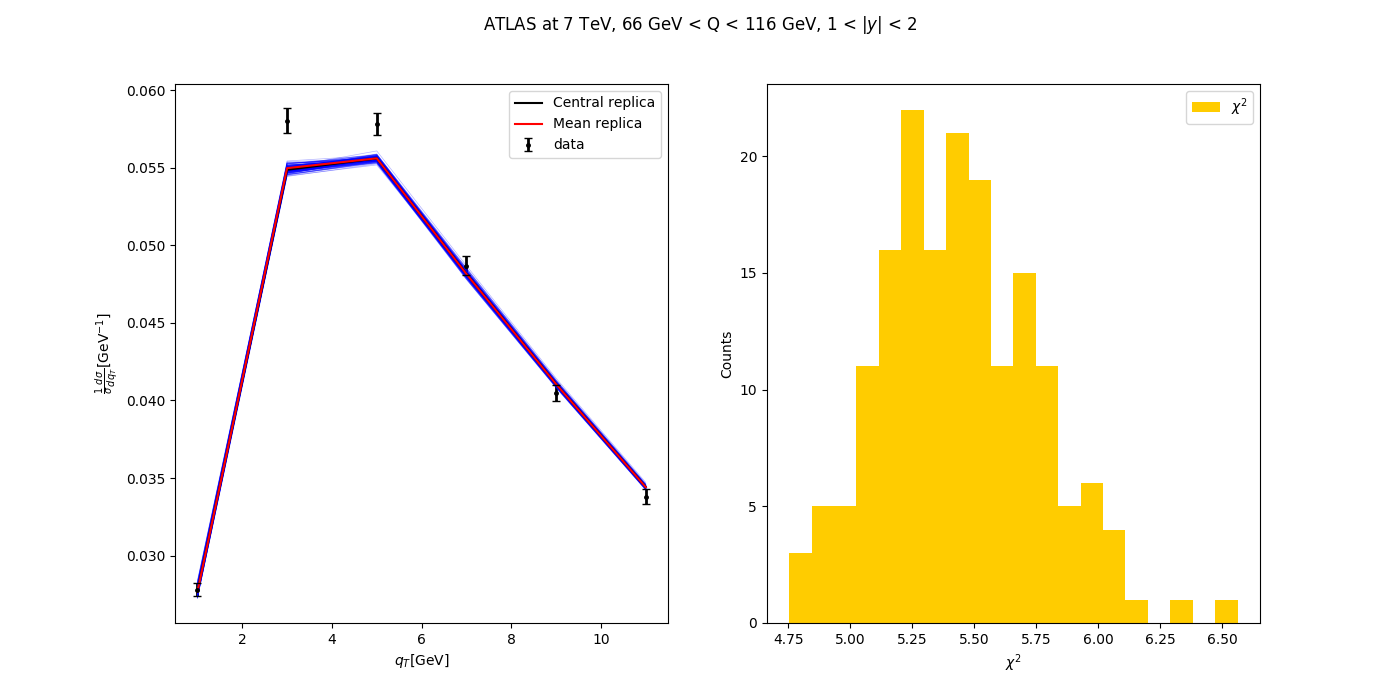
\includegraphics{pngplots/ATLAS_7TeV_y_1_2.png}
\caption{ATLAS\_7TeV\_y\_1\_2 data-theory comparison}
\end{figure}

\begin{figure}
\centering
\includegraphics{pngplots/ATLAS_7TeV_y_2_2.4.png}
\caption{ATLAS\_7TeV\_y\_2\_2.4 data-theory comparison}
\end{figure}

\begin{figure}
\centering
\includegraphics{pngplots/ATLAS_8TeV_y_0_0.4.png}
\caption{ATLAS\_8TeV\_y\_0\_0.4 data-theory comparison}
\end{figure}

\begin{figure}
\centering
\includegraphics{pngplots/ATLAS_8TeV_y_0.4_0.8.png}
\caption{ATLAS\_8TeV\_y\_0.4\_0.8 data-theory comparison}
\end{figure}

\begin{figure}
\centering
\includegraphics{pngplots/ATLAS_8TeV_y_0.8_1.2.png}
\caption{ATLAS\_8TeV\_y\_0.8\_1.2 data-theory comparison}
\end{figure}

\begin{figure}
\centering
\includegraphics{pngplots/ATLAS_8TeV_y_1.2_1.6.png}
\caption{ATLAS\_8TeV\_y\_1.2\_1.6 data-theory comparison}
\end{figure}

\begin{figure}
\centering
\includegraphics{pngplots/ATLAS_8TeV_y_1.6_2.png}
\caption{ATLAS\_8TeV\_y\_1.6\_2 data-theory comparison}
\end{figure}

\begin{figure}
\centering
\includegraphics{pngplots/ATLAS_8TeV_y_2_2.4.png}
\caption{ATLAS\_8TeV\_y\_2\_2.4 data-theory comparison}
\end{figure}

\begin{figure}
\centering
\includegraphics{pngplots/ATLAS_8TeV_Q_46_66.png}
\caption{ATLAS\_8TeV\_Q\_46\_66 data-theory comparison}
\end{figure}

\begin{figure}
\centering
\includegraphics{pngplots/ATLAS_8TeV_Q_116_150.png}
\caption{ATLAS\_8TeV\_Q\_116\_150 data-theory comparison}
\end{figure}

\end{document}
